\chapter{Base de datos bio-ópticos de campo}
\label{dat}

\section{Introducción}
\label{dat:s:intro}

    La factibilidad y el poder predictivo de la mayoría de los algoritmos de estimación de variables biogeofísicas a partir de sensores remotos de color reside en gran parte en la disponibilidad de mediciones de campo de buena calidad de dichas variables. En general, tanto el alcance espacial como la plausibilidad de dichos algoritmos dependerá de la representatividad geográfica, la calidad y la cantidad de datos de campo que se disponga, por lo que el número total de mediciones requeridas suele ser grande. Esto implica que es fundamental mantener nuestro conjunto de datos de manera sistematizada y accesible.
    
    Una parte fundamental del trabajo de esta tesis consistió en adquirir, procesar y analizar datos de campo adquiridos principalmente en el estuario del Río de la Plata (RdP), aunque también en otras regiones. El volumen de datos de campo bio-ópticos disponibles para la región fue creciendo considerablemente desde el inicio de la presente tesis (los primeros datos radiométricos disponibles para la región corresponden a octubre del año 2012, medidos desde el Muelle del Club de Pescadores de Palermo, Buenos Aires), por lo que una tarea fundamental fue continuar con las tareas de campo y sistematizar la información obtenida en una base de datos. Si bien parte de estos datos fueron utilizados para el desarrollo de esta tesis, su recolección y sistematización trasciende los fines específicos de la misma, dado que dicha información es y será utilizada para continuar avanzando en la comprensión y el diseño de nuevos algoritmos en las aguas ópticamente complejas del estuario del RdP, así como de otras regiones de estudio que conforman parte de la base de datos.
    
    En este capítulo se describirán y analizarán las mediciones de campo realizadas en el marco de esta tesis, las cuales se realizaron durante campañas que perseguían objetivos específicos, ya sea en el marco de convenios o proyectos científicos o bien con la intención de documentar un evento puntual (por ejemplo, la invasión de plantas acuáticas superficiales en el verano de 2015/2016 en el RdP, \S \ref{cam}). En primer lugar, se describirán las áreas de estudio, los instrumentos utilizados, sus protocolos de medición y adquisición, sus protocolos de procesamiento y los criterios utilizados para la conformación de una base de datos sistematizada. Por otro lado, se analizará el comportamiento global obtenido para las principales variables bioópticas medidas en el RdP y se las comparará con los valores medidos en otras áreas estudiadas, cuyas aguas también son ópticamente complejas: el estuario del Río Tajo (Portugal) y la Laguna de Chascomús, en la Provincia de Buenos Aires.
   
\section{Características generales de las campañas}
\label{dat:s:generales}

    Durante las campañas se realizaron dos tipos de mediciones según su carácter temporal: o bien i) se midió de forma continua desde el inicio hasta el final de cada jornada de medición (por ejemplo, con el turbidímetro OBS501, ver \S \ref{dat:s:obs}), o bien ii) en forma discreta (estaciones) en horarios preestablecidos. Por otro lado, los horarios de las estaciones se determinaron fundamentamente (aunque no en todos los casos) siguiendo dos criterios fundamentales:
    
          \begin{itemize}
            \item La selección de fechas de medición depende fundamentalmente de i) las condiciones meteorológicas y ii) las pasadas de diferentes satélites de interés.
            \item  Generalmente se trata de realizar una estación simultánea para cada horario de adquisición de las imágenes satelitales de interés que estén disponibles para la jornada de medición. Dichas estaciones son las más relevantes para la validación de productos biogeofísicos satelitales (ejercicio de \textit{match up}).
            \item Fuera de los horarios de las pasadas se intentó generalmente que las estaciones se realizaran de manera periódica para intentar captar la variabilidad diaria del sitio durante la jornada de muestreo. Aún así, es en general impracticable obtener una periodicidad exacta para el muestreo por estación, dado que existen diversas causas de retrasos o adelantos en los tiempos de medición (advenimiento de una nube que perjudique las mediciones radiométricas, falla temporal de algún sensor, desperdicios flotantes en el agua que es necesario remover, etc.).
        \end{itemize}

\section{Áreas de estudio}
\label{dat:s:areas}

    Si bien la gran mayoría de las campañas realizadas como parte de la presente tesis - o bien dentro de nuestro grupo de investigación - tuvieron lugar en distintas regiones del RdP (descrito en \S \ref{int:s:area}), la base de datos total comprende información recopilada de varias otras regiones: los estuarios de los ríos Escalda (Bélgica), Girondo (Francia) y Tajo (Portugal), los golfos patagónicos de San Matías y San Jorge, la Estación Permanente de Estudios Ambientales (EPEA) frente a Mar del Plata y diversas lagunas bonaerenses. En el presente capítulo nos limitaremos a describir los resultados de los datos medidos en el RdP (Figuras \ref{dat:bardp} y \ref{dat:caba}) y a compararlos con el siguiente subconjunto de sitios:
    
    \begin{itemize}
    \item \textbf{Estuario del Río Tajo}: El estuario del Río Tajo se ubica en la costa oeste de Portugal y atraviesa la región urbana de su capital, Lisboa (Figura \ref{dat:tagus}). Cubre aproximadamente 320 km$^{2}$ y conforma una cuenca somera dominada por efecto de la marea que conecta con el Océano Atlántico mediante una profunda y estrecha entrada mareal (Guerreiro et al. 2015, \cite{guerreiro2015}). El lecho del estuario está compuesto principalmente por arenas y arcillas, ambas de origen fluvial y local; mientras que la boca y el canal intermareal están dominados por arenas de origen marino (Freire et al. 2007, \cite{freire2007}). Este estuario comparte con el RdP la característica de que sus aguas están ópticamente dominadas por la presencia de sedimentos inorgánicos en suspensión, aunque, a diferencia del RdP, las concentraciones de sedimentos son más bien moderadas. A su vez, suele presentar una fracción de material orgánico mayor a la del RdP. Estas similitudes y diferencias hacen interesante la comparación del comportamiento general de las variables bioópticas medidas en ambos estuarios.
    \item \textbf{Laguna de Chascomús}: la Laguna de Chascomús (Figura \ref{dat:chascomus}) es un cuerpo de agua turbia (hasta 300 FNU) debido a las altas concentraciones de fitoplancton (algas unicelulares, principalmente de los grupos de las cianobacetrias, \textit{Chlorophyceae} y \textit{Bacillariophyceae}) y material inorgánico (Sánchez et al. 2019, \cite{sanchez2018}). A diferencia del RdP, cuya aguas suelen presentar bajas concentraciones de fitoplancton, es de esperar que las reflectancias medidas en esta laguna presenten rasgos espectrales asociados a la absorción de los principales pigmentos que abundan en las células de dichos organismos.
    \end{itemize}
    
    \begin{figure}
    \centering
    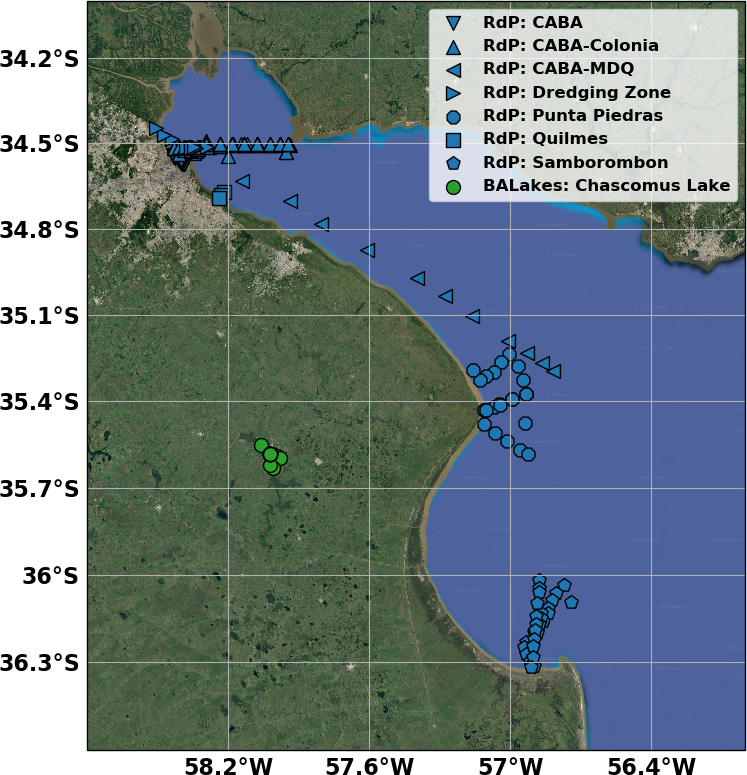
\includegraphics[width=\textwidth]{dat/figures/MAP_BARdp.png}
    \caption[Ubicación de las estaciones de campañas en la Provincia de Buenos Aires y el RdP.]{Ubicación de las estaciones de campañas en la Provincia de Buenos Aires y el RdP. El mapa resulta de una proyección \textit{Plate Carrée} del mosaico utilizado por la aplicación Google Maps, resultante de un ensamblado de representaciones RGB de imágenes ópticas de diversos satelites estadounidenses (de la serie LandSat) y europeos (del progama Copernicus). Naturalmente, el color azulado que se observa sobre el RdP no corresponde al color observado desde el espacio, sino que proviene de una máscara aplicada por Google Maps.}
    \label{dat:bardp}
    \end{figure}
    
    \begin{figure}
    \centering
    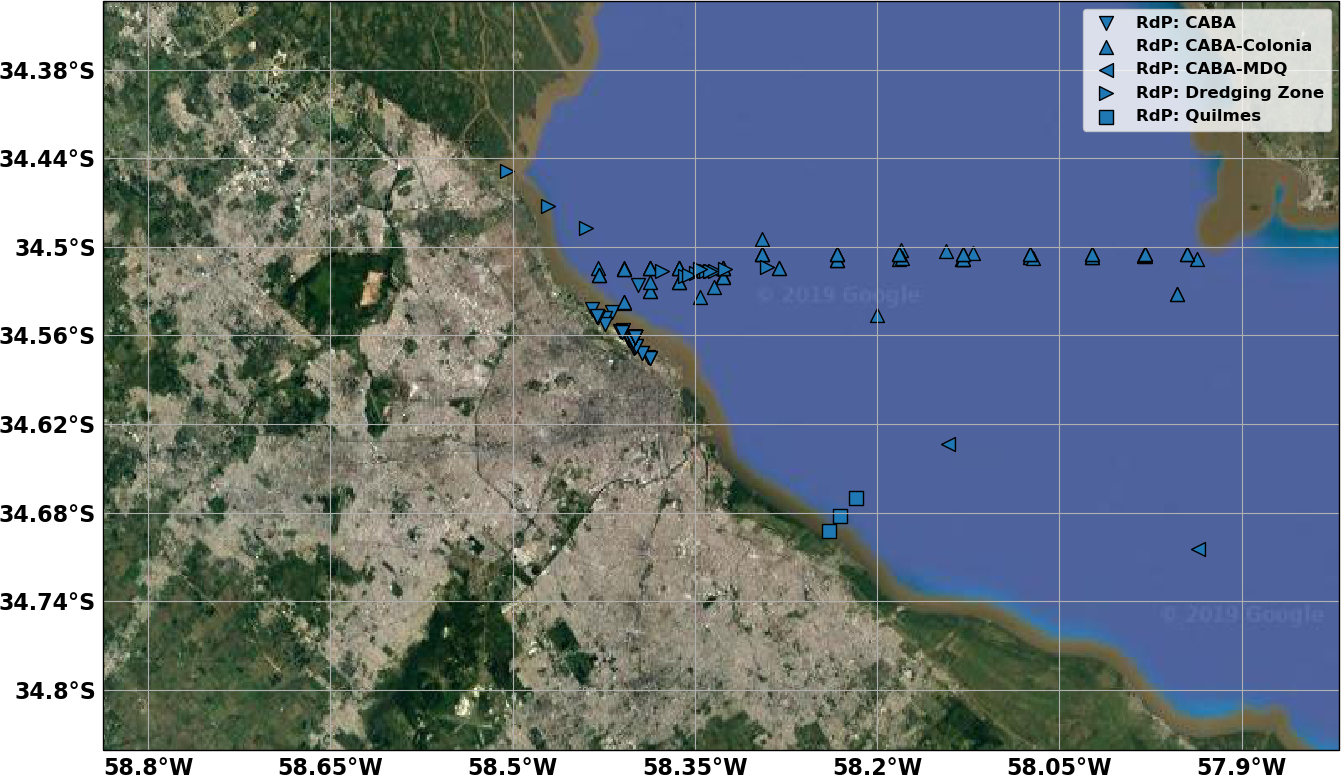
\includegraphics[width=\textwidth]{dat/figures/MAP_CABA.png}
    \caption[Ubicación de las estaciones de campañas en la región de la Ciudad de Buenos Aires.]{Ídem Figura \ref{dat:bardp}, ampliado en la región de la Ciudad de Buenos Aires.}
    \label{dat:caba}
    \end{figure}
    
    
    \begin{figure}
    \centering
    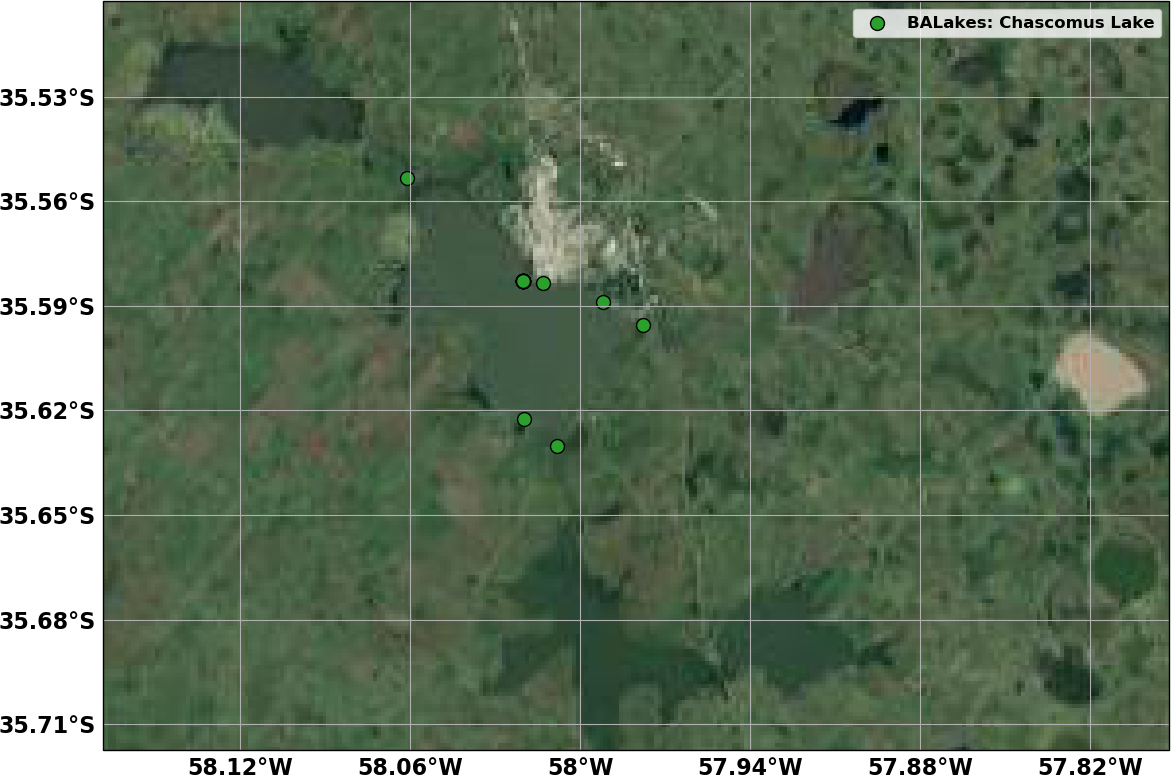
\includegraphics[width=\textwidth]{dat/figures/MAP_Chascomus.png}
    \caption[Ubicación de las estaciones de campañas en la región de la Laguna de Chascomús.]{Ídem Figura \ref{dat:bardp}, ampliado en la región de la Laguna de Chascomús (Chascomús, Prov. Buenos Aires).}
    \label{dat:chascomus}
    \end{figure}
    
    \begin{figure}
    \centering
    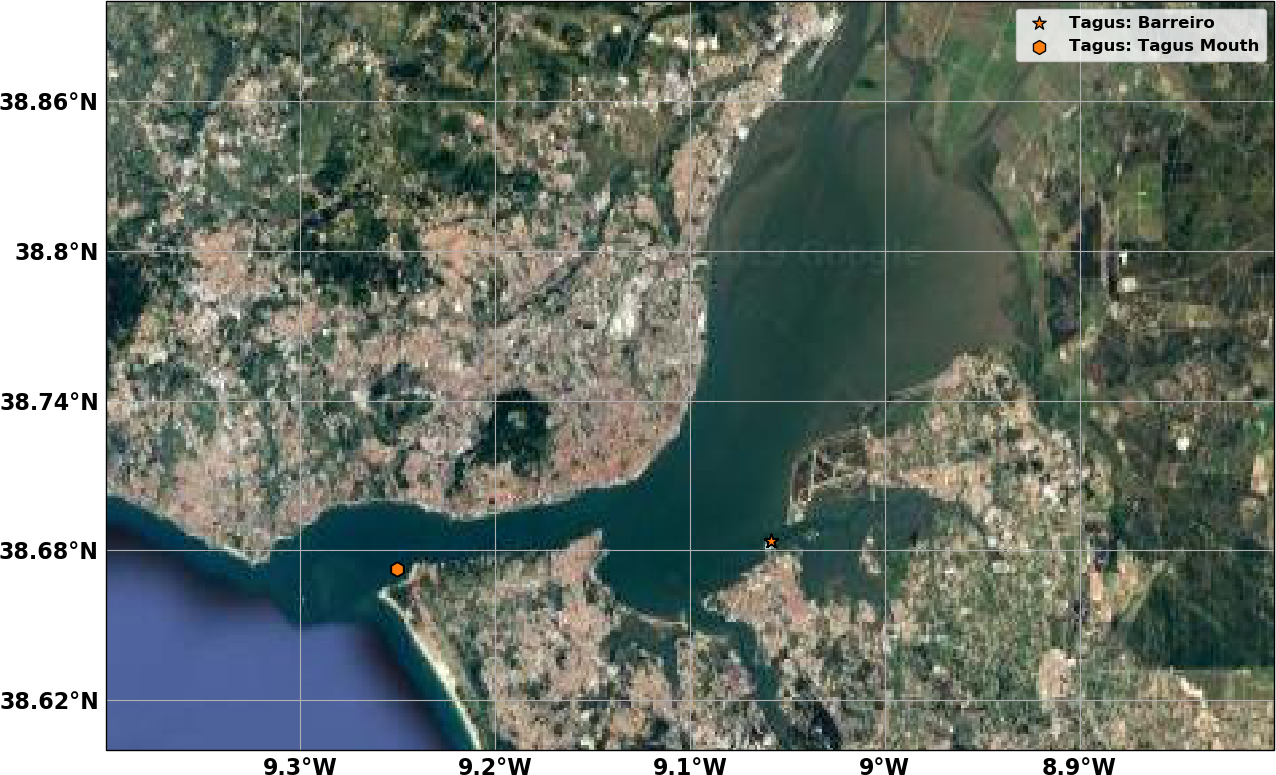
\includegraphics[width=\textwidth]{dat/figures/MAP_Tagus.png}
    \caption[Ubicación de las estaciones de campañas en la región del Estuario del Río Tajo (Portugal).]{Ídem Figura \ref{dat:bardp}, pero para las estaciones de campañas en el Estuario del Río Tajo (Lisboa, Portugal).}
    \label{dat:tagus}
    \end{figure}
    
    El Cuadro \ref{dat:tab:inventario} resume las campañas e instrumentos considerados en el presente capítulo [mediciones de la base de datos realizadas en otras regiones o con otros instrumentos fueron omitidas por exceder los objetivos de la presente tesis]. Obsérvese que los códigos identificatorios de cada campaña siguen el formato Región\_aaaammdd (año-mes-día), y que las siglas \textit{RdP}, \textit{BALakes} y \textit{Tagus} son los códigos identificatorios del RdP, las lagunas bonaerenses (dentro de las cuales se halla la de Chascomús) y el Río Tajo, respectivamente. A su vez, el Cuadro \ref{dat:tab:siglas} hace una breve descripción de las mediciones consideradas.
    
    \begin{table}
    \caption[Inventario del subconjunto de campañas analizado.]{Inventario del subconjunto de campañas caracterizado y analizado en este capítulo. Número de estaciones realizadas para cada uno de los instrumentos utilizados en cada una de las campañas [ver Cuadro \ref{dat:tab:siglas} para una breve descripción de cada instrumento].}
    \small
    \begin{tabular}{|l|c|c|c|c|c|}
    \hline
    \textbf{ID de campaña}                            & \textbf{ASD}             & \textbf{Trios}           & \textbf{OBS501}          & \textbf{SPM}             & \textbf{HACH}            \\ \hline
    \textbf{Región\_yyyymmdd}                         & \cellcolor[HTML]{000000} & \cellcolor[HTML]{000000} & \cellcolor[HTML]{000000} & \cellcolor[HTML]{000000} & \cellcolor[HTML]{000000} \\ \hline
    {\color[HTML]{009901} \textbf{BALakes\_20170131}} &                          & 1                        & 5                        & 1                        & 8                        \\ \hline
    {\color[HTML]{009901} \textbf{BALakes\_20170504}} &                          & 5                        & 5                        & 2                        & 3                        \\ \hline
    {\color[HTML]{009901} \textbf{BALakes\_20180409}} &                          & 5                        & 5                        & 5                        & 5                        \\ \hline
    {\color[HTML]{009901} \textbf{BALakes\_20190321}} &                          & 9                        & 11                       & 2                        & 11                       \\ \hline
    {\color[HTML]{3166FF} \textbf{RdP\_20120515}}     &                          &                          &                          & 13                       &                          \\ \hline
    {\color[HTML]{3166FF} \textbf{RdP\_20121018}}     &                          &                          &                          &                          & 10                       \\ \hline
    {\color[HTML]{3166FF} \textbf{RdP\_20121031}}     &                          &                          &                          &                          & 5                        \\ \hline
    {\color[HTML]{3166FF} \textbf{RdP\_20121101}}     & 3                        &                          &                          &                          & 3                        \\ \hline
    {\color[HTML]{3166FF} \textbf{RdP\_20121113}}     & 37                       &                          &                          & 70                       & 89                       \\ \hline
    {\color[HTML]{3166FF} \textbf{RdP\_20130123}}     & 8                        &                          &                          &                          & 7                        \\ \hline
    {\color[HTML]{3166FF} \textbf{RdP\_20130227}}     & 11                       &                          &                          & 11                       & 11                       \\ \hline
    {\color[HTML]{3166FF} \textbf{RdP\_20130416}}     & 11                       &                          &                          &                          & 11                       \\ \hline
    {\color[HTML]{3166FF} \textbf{RdP\_20130430}}     & 11                       &                          &                          & 13                       & 12                       \\ \hline
    {\color[HTML]{3166FF} \textbf{RdP\_20131120}}     & 1                        &                          &                          & 3                        & 3                        \\ \hline
    {\color[HTML]{3166FF} \textbf{RdP\_20131220}}     & 5                        &                          &                          & 5                        & 13                       \\ \hline
    {\color[HTML]{3166FF} \textbf{RdP\_20140106}}     & 3                        &                          &                          & 5                        & 12                       \\ \hline
    {\color[HTML]{3166FF} \textbf{RdP\_20140227}}     &                          &                          &                          & 5                        & 12                       \\ \hline
    {\color[HTML]{3166FF} \textbf{RdP\_20140318}}     & 3                        &                          &                          & 2                        & 13                       \\ \hline
    {\color[HTML]{3166FF} \textbf{RdP\_20140411}}     &                          &                          &                          & 2                        & 8                        \\ \hline
    {\color[HTML]{3166FF} \textbf{RdP\_20140415}}     & 9                        &                          &                          & 4                        & 9                        \\ \hline
    {\color[HTML]{3166FF} \textbf{RdP\_20140501}}     & 4                        &                          &                          & 5                        & 15                       \\ \hline
    {\color[HTML]{3166FF} \textbf{RdP\_20140516}}     & 4                        &                          &                          & 2                        & 9                        \\ \hline
    {\color[HTML]{3166FF} \textbf{RdP\_20140619}}     & 5                        &                          &                          & 5                        & 13                       \\ \hline
    {\color[HTML]{3166FF} \textbf{RdP\_20140819}}     &                          &                          &                          & 7                        & 15                       \\ \hline
    {\color[HTML]{3166FF} \textbf{RdP\_20141122}}     & 6                        &                          &                          & 8                        & 8                        \\ \hline
    {\color[HTML]{3166FF} \textbf{RdP\_20141217}}     &                          &                          &                          &                          & 9                        \\ \hline
    {\color[HTML]{3166FF} \textbf{RdP\_20150423}}     & 12                       &                          &                          &                          & 4                        \\ \hline
    {\color[HTML]{3166FF} \textbf{RdP\_20151118}}     &                          & 16                       &                          &                          & 42                       \\ \hline
    {\color[HTML]{3166FF} \textbf{RdP\_20160421}}     &                          &                          &                          &                          & 8                        \\ \hline
    {\color[HTML]{3166FF} \textbf{RdP\_20160925}}     &                          & 7                        &                          & 15                       & 15                       \\ \hline
    {\color[HTML]{3166FF} \textbf{RdP\_20170106}}     &                          & 4                        &                          &                          & 4                        \\ \hline
    {\color[HTML]{3166FF} \textbf{RdP\_20170126}}     &                          & 3                        &                          &                          & 16                       \\ \hline
    {\color[HTML]{3166FF} \textbf{RdP\_20180404}}     &                          & 16                       & 22                       & 10                       & 22                       \\ \hline
    {\color[HTML]{3166FF} \textbf{RdP\_20181105}}     &                          & 29                       & 33                       & 17                       & 33                       \\ \hline
    {\color[HTML]{3166FF} \textbf{RdP\_20181202}}     &                          & 7                        & 7                        & 11                       & 11                       \\ \hline
    {\color[HTML]{3166FF} \textbf{RdP\_20190923}}     &                          &                          &                          & 5                        &                          \\ \hline
    {\color[HTML]{FFC702} \textbf{Tagus\_20180828}}   &                          & 27                       &                          & 22                       & 26                       \\ \hline
    {\color[HTML]{FFC702} \textbf{Tagus\_20190617}}   &                          & 22                       &                          &                          & 20                       \\ \hline
    \end{tabular}
    \label{dat:tab:inventario}
    \end{table}
    
    \begin{table}
    \caption[Descripción breve de las variables de campo medidas, caracterizadas y analizadas.]{Descripción breve de las variables de campo medidas, caracterizadas y analizadas en el presente capítulo.}
    \small
    \begin{tabular}{|l|l|l|}
    \hline
    \textbf{Sigla} & \textbf{Descripción breve} & \textbf{Referencia} \\ \hline
    \textbf{ASD} & Espectroradiómetro hiperespectral, rango {[}350 - 2500{]} nm & Knaeps et al. 2012 \cite{knaeps2012} \\ \hline
    \textbf{TriOS} & Espectroradiómetro hiperespectral, rango {[}350 - 950{]} nm & Tilstone et al. 2001 \cite{tilstone2001}   \\ \hline
    \textbf{HACH}  & Turbidímetro portátil (nefelómetro + transmisómetro) & Dogliotti et al. 2015 \cite{dogliotti2015} \\ \hline
    \textbf{OBS}   & \begin{tabular}[c]{@{}l@{}} Medidores de turbidez en continuo \\ (nefelómetro \textit{SS\_OBS501} y retrodispersómetro \textit{BS\_OBS501})\end{tabular} & Campbell Scientific \cite{campbell}\\ \hline
    \textbf{SPM}   & \begin{tabular}[c]{@{}l@{}}Determinación de Material Particulado en Suspensión \\ (orgánico, inorgánico y total) mediante método gravimétrico\end{tabular} & Tilstone et al. 2001 \cite{tilstone2001}   \\ \hline
    \end{tabular}
    \label{dat:tab:siglas}
    \end{table}

\section{Mediciones radiométricas (ASD y TriOS)}
\label{dat:s:radiometricas}
    Las mediciones radiométricas son las más críticas dado que se realizan con sensores ópticos pasivos (al igual que los sensores ópticos de color del mar) y su calidad depende fuertemente de las cualidades \textit{aparentes} de la radiancia ingresante al sensor. Para obtener reflectancias de buena calidad es necesario tener en cuenta que:
    \begin{itemize}
        \item Son preferibles condiciones de nubosidad estable, es decir, o bien cielo totalmente despejado, o bien totalmente cubierto (aunque en este último caso, naturalmente, no será posible realizar \textit{match ups}).
        \item En caso de presentarse nubosidad variable, es fundamental chequear que no haya obstrucciones intermitentes del limbo solar durante las mediciones.
        \item Es importante evitar que el cono visual de cada uno de los sensores en cuestión no esté afectado por sombras u obstáculos (e.g. objetos flotantes locales).
        \item Las mediciones deben realizarse, dentro de lo posible, con ángulos cenitales solares menores a $60 \degree$.
    \end{itemize}
    
    En las campañas se  han utilizado dos radiómetros diferentes para medir la radiación fuera del agua:\footnote{Cabe mencionar que tambien pueden ser utilizados dentro del agua, pero dadas las carecteríticas altamente absortivas de las aguas ópticamente complejas estudiadas la metodología \textit{above-water} es la recomendada (Ruddick et al. 2019, \cite{ruddick2019}).}
    \begin{itemize}
        \item El espectroradiómetro Analytic Spectral Devices (ASD FieldSpec FR) que funciona en el rango espectral 350-2500 nm con una resolución espectral de 3 nm entre 350 nm y 900 nm y entre 10 nm y 12 nm en la región del infrarojo de onda corta (900-2500 nm). Se utilizó un paso de discretización de 1 nm.
        \item El sistema RAMSES/TriOS, conformado por dos radiómetros y un irradiómetro hiperespectrales que funcionan en el rango 350-950 nm, con una resolución espectral de 3.3 nm. Se utilizó un paso de discretización de 2.5 nm.
    \end{itemize}
    
    Para poder calcular la reflectancia espectral del agua, $\rho_{w}$ (Ec. \ref{int:eq:reflectancia})) utilizando radiómetros fuera del agua es necesario adquirir mediciones directas de tres variables radiométricas: la radiancia ascendente ($L_{u}$, proveniente del agua, Ec. \ref{int:eq:radiancia}), la radiancia descendente ($L_{sky}$, proveniente del cielo en ángulo reflejado respecto de la horizontal a la medición de $L_{u}$) y la irradiancia descendente ($E_{d}$, proveniente de todos los ángulos de observación superiores al plano horizontal, Ec. \ref{int:eq:irradiancia}). Para estas mediciones es fundamental mantener una geometría de observación-iluminación adecuada de forma tal de garantizar que la radiancia entrante al sensor sea la requerida al momento de computar la reflectancia del agua. Los ángulos cenital y acimutal utilizados para cada una de las variables se especifican en el Cuadro \ref{dat:tab:radiometria} y en las Figuras \ref{dat:ASD} y \ref{dat:TriOS}.
    
    Con ambos radiómetros, se midieron $L_{u}$ y $L_{sky}$ con un azimut relativo al sol de $135 \degree$ ó $ 90 \degree$ y ángulos horizontales recíprocos de $\theta = \pm 50\degree$ ) (ángulos de acuerdo con Mueller et al. 2003, \cite{mueller2003}). La irradiancia $E_{d}$ es medida por el irradiómetro apuntando al cenit, en el caso del TriOS, mientras que en el caso del ASD la fibra óptica se apunta hacia el nadir sobre una placa cuasi-lambertiana calibrada y se multiplica el valor medido por $\pi$ (asumiendo que la placa es un emisor coseno).
    %
    El protocolo de medición del ASD se detalla en Knaeps et al. 2012, \cite{knaeps2012}, y sigue el \textit{Método 2 por encima del agua} genérico de los Protocolos de Óptica del Océano 2003 de la NASA (Mueller et al. 2003, \cite{mueller2003}); mientras que el protocolo de medición con el sistema TriOS se detalla en Tilstone et al. 2001, \cite{tilstone2001}.
    %
    Las Figuras \ref{dat:ASD} y \ref{dat:TriOS} muestran la disposición de sendos radiómetros. A su vez, los ángulos de observación de ambos sensores se hallan resumidos en el Cuadro \ref{dat:tab:radiometria}
    

    \begin{table}
    \caption{Ángulos e instrumentos de medición según magnitud a medir y dispositivo utilizado.}
    \small
    \begin{tabular}{|l|l|l|l|}
    \hline
    \textbf{Nombre}                   & \textbf{\begin{tabular}[c]{@{}l@{}}Ángulo\\ horizontal\end{tabular}}                & \textbf{\begin{tabular}[c]{@{}l@{}}Acimut\\ relativo\end{tabular}} & \textbf{Instrumento} \\ \hline
    Radiancia ascendente ($L_{u}$)    & $-50 \degree$                                                                       & $90 \degree - 135 \degree$                                         & Radiómetro\\ \hline
    Radiancia del cielo ($L_{sky}$)   & $50 \degree$                                                                        & $90 \degree - 135 \degree$                                         & Radiómetro\\ \hline
    Irradiancia descendente ($E_{d}$) & \begin{tabular}[c]{@{}l@{}}TriOS: $ 90 \degree $\\ ASD: $-90 \degree $\end{tabular} & - & \begin{tabular}[c]{@{}l@{}}TriOS: Irradiómetro\\ ASD: Radiómetro s/ Spectralon\end{tabular} \\ \hline
    \end{tabular}
    \label{dat:tab:radiometria}
    \end{table}

    Las mediciones de $L_{u}$, $E_{d}$ y $L_{sky}$ se utilizan para calcular la reflectancia del agua sobre la superficie, $\rho_{w}$:

    \begin{equation}
        \rho_{w}(\lambda) = \pi \frac{L_{u}(\lambda)-\rho_{sky}(w)L_{sky}(\lambda)}{E_{d}(\lambda)}
        \label{dat:eq:rhoWField}
    \end{equation}

    \noindent
    donde $\rho_{sky}$ es el coeficiente de Fresnel para la radiancia tomado de Mobley 1999, \cite{mobley1999}.
    %    
    En general, se espera que este coeficiente varíe en función de la velocidad del viento (debido a que este perturba la geometría - \textit{a priori} plana - de la interfase) en condiciones de cielo despejado, pero que sea casi independiente del viento en condiciones de cielo totalmente cubierto por nubes. Esto se puede tener en cuenta evaluando la cobertura nubosa mediante la relación $L_{sky}/E_{d}$ en 750 nm, la cual puede tener valores de 0.02 en condiciones de cielo claro (Mobley 1999, \cite{mobley1999}), pero que presenta valores mayores (e.g. del orden de 0.3 para cielos $100\%$ nublados). De esta forma $\rho_{sky}$ se puede calcular según lo explicitado en Ruddick et al. 2006 \cite{ruddick2006}:
    
    \begin{equation}
    \begin{aligned}
        \frac{L_{sky}(750)}{E_{d}(750)} < 0.05 \rightarrow \rho_{sky} & = 0.0256 + 0.00039 w + 0.000034 w^{2}\\
        \frac{L_{sky}(750)}{E_{d}(750)} \geq 0.05 \rightarrow \rho_{sky} & = 0.0256
    \end{aligned}
    \label{dat:eq:mobley}
    \end{equation}
    
    \noindent
    donde $w$ es la velocidad del viento en superficie en $m/s$. En algunos casos de mediciones costeras, como las realizadas desde el Muelle de Pescadores de Palermo se consideró viento igual a cero ($w=0$) en la Ec. \ref{dat:eq:mobley} debido a que en estos sitios costeros la parametrización de la rugosidad de la superficie en función del viento utilizada se aparta fuertemente de la realidad.
    
    Una vez obtenidas las reflectancias espectrales, y habiendo aplicado los pasos de procesamiento específicos a cada sensor (detallados en las siguientes subsecciones) es posible aplicar una corrección para eliminar el \textit{sunglint} residual que consiste en sustraer un sesgo espectralmente blanco a una longitud de onda dada, $\lambda_{0}$:
    
    \begin{equation}                
        \rho_{w}(\lambda) = \rho_{w}(\lambda) - \rho_{w}(\lambda_{0})
    \end{equation}
    
    El supuesto subyacente en esta sustracción es que la señal proveniente del agua es nula a $\lambda_{0}$. En el caso de ASD, siempre se usa $\lambda_{0} = 1305$ nm ya que a esta longitud de onda siempre se espera una señal del agua nula debido a que la absorción de agua pura es extremadamente alta (Kou et al. 1993, \cite{kou1993}, Pope y Fry 1997, \cite{pope1997}). En el caso de TriOS se puede usar opcionalmente $\lambda_{0} = 900$ nm  sólo si el contenido de partículas no es demasiado alto y en caso de detectar un desplazamiento espectralmente blanco en la señal que está asociada al ingreso de \textit{sunglint} moderado. Esto también suele ser observable en fotografías simultáneas tomadas al momento de medir.

    % This can be done as a way to correct for some moderate sunglint that affected the measurements. We assumed here that the in-water signal was 0 at 900 nm, since the turbidity was not too high for none of the stations of this campaign. In the case of ASD, $\lambda_{0} = 1305 nm$ is always used since at this wavelength it is always expected to have no signal from the water due to extremely high pure water absorption. In the case of TriOS, only if the particle content is not too high, $\lambda_{0} = 900 nm$ can be optionally used in case of detecting a white offset at the signal that is evidently associated to some moderate sunglint (also observable from simultaneous pictures of the scene).
    
    % Additionaly, in some cases, we apply:
    % \begin{equation}
    %     max{CV(\rho_{w}(400:900 nm))} < 20 \%.
    % \end{equation}
    % This is equivalent to force the CV to be lower than 20\% throughout the range 400-900 nm. But this isn't satisfied for stations where the mean values at the NIR are too small, and they become indistinguishable from the sensor noise.
    
    Más allá de los criterios de control de calidad específicos a cada tipo de sensor - detallados en las siguientes secciones - se suele imponer un control de calidad sobre el coeficiente de variación del espectro (CV):

    \begin{equation}
    \begin{aligned}
        max\{CV(\rho_{w}(400:900 nm))\} < 20 \%.\\
        CV(\rho_{w}(\lambda_{0})) < 20\%
    \end{aligned}    
    \label{dat:eq:CV}
    \end{equation}
    
    \noindent donde la primera condición es equivalente a forzar el coeficiente de variación (CV) a ser menor al 20\% a lo largo del rango 400-900 nm, y la segunda condición se calcula sobre alguna longitud de onda en el SWIR, según sea conveniente/posible. Estas condiciones no se aplican globalmente en los controles de calidad dado que existen estaciones donde los valores medidos en el NIR/SWIR son demasiado bajos y caen por debajo del umbral de ruido del sensor.
    
    
    \begin{figure}
    \centering
    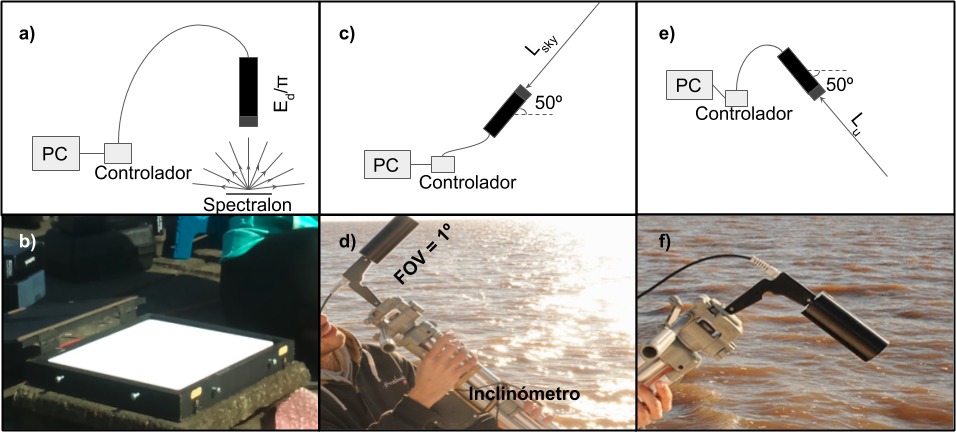
\includegraphics[width=\textwidth]{dat/figures/ASD.png}
    \caption[Disposición del radiómetro ASD utilizada para las mediciones.]{Disposición del radiómetro ASD utilizada para las mediciones. La geometría de sensado se regula mediante un trípode y un inclinómetro. Esquemas de la adquisicón de la irradiancia descendente, $E_{d}$ (a), radiancia ascendente, $L_{u}$ (c) y radiancia del cielo en ángulo horizontal recíproco a $L_{u}$, $L_{sky}$ (e). b),d),f): Fotografías correspondientes a cada una de estas geometrías, campaña RdP\_20140617.}
    \label{dat:ASD}
    \end{figure}

    \subsection{Radiómetro ASD}
    \label{dat:s:asd}
    
        El ASD es un radiómetro hiperespectral de campo en el rango 350-2500 nm cuya geometría de adquisición es regulada por una fibra óptica. El ASD utilizado para llevar a cabo las mediciones que conforman parte de nuestra base de datos pertenece a la CONAE (Comisión Nacional de Actividades Espaciales).

        \subsubsection{ASD: Protocolo de medición}
        \label{dat:s:asdMed}

            La metodología de medición se basa en los protocolos desarrollados y recomendados por la NASA (Mueller et al., 2000 \cite{mueller2003}). Se utilizó una lente con un ángulo de observación (\textit{Field of View} - FOV) de $1 \degree$, la configuración geométrica se describe en la Figura \ref{dat:ASD}, el Cuadro \ref{dat:tab:radiometria} y la configuración del equipo es detallada Dogliotti et al. 2014 \cite{dogliotti2014}.

            Se realizan tres series de mediciones sucesivas en la siguiente secuencia: $E_{d}$, $L_{u}$, $L_{sky}$, $L_{u}$, $L_{sky}$, $L_{u}$, $L_{sky}$, totalizando 21 mediciones (Cuadro \ref{dat:tab:asd}). En cada una de estas será necesario establecer un tiempo de integración del sensor.
            \begin{table}
            \caption{Orden consecutivo de las mediciones realizadas por el espectrorradiómetro ASD durante cada estación.}
                \begin{tabular}{|l|l|l|l|l|l|l|l|}
                \hline
                 & $E_{d}$ & $L_{u}$ & $L_{sky}$ & $L_{u}$ & $L_{sky}$ & $L_{u}$ & $L_{sky}$ \\ \hline
                1$^{ra}$ Serie & 1 & 2 & 3 & 4 & 5 & 6 & 7 \\ \hline
                2$^{da}$ Serie & 8 & 9 & 10 & 11 & 12 & 13 & 14 \\ \hline
                3$^{ra}$ Serie & 15 & 16 & 17 & 18 & 19 & 20 & 21 \\ \hline
                \end{tabular}
            \label{dat:tab:asd}
            \end{table}

        \subsubsection{ASD: Protocolo de procesamiento}
        \label{dat:s:asdProc}
        
            El cálculo de la reflectancia del agua se obtiene de promediar los 9 escaneos - resultantes de los tres escaneos de $L_{u}$ y $L_{sky}$ para cada una de las tres series - obtenidos para la reflectancia (Ec. \ref{dat:eq:rhoWField}), aunque previamente se consideran una serie de criterios para garantizar la obtención de buenas mediciones (estabilidad de $E_{d}$, detección de anomalías y control del desvío estándar en las reflectancias) sobre 4 longitudes de onda en el rango VIS-NIR: $\lambda_{0}$ = 450 nm, 600 nm, 750 nm y 900 nm. Estas longitudes de onda,  distribuidas cada 150 nm, fueron elegidas para que cubran todo el rango de interés y haya solapamiento con las longitudes de onda utilizadas en el protocolo utilizado previamente ($750$ y $900\sim930$ nm). El código de procesamiento fue hecho para que la elección de estas longitudes de onda y los umbrales de los respectivos criterios puedan tomarse como entradas fáciles de modificar. La Figura \ref{dat:ASD_QC} muestra cómo se aplicaron dichos criterios a los escaneos de la estación RdP\_20131220\_DCAO-E.
            
            A continuación se enumeran y describen los criterios de calidad mencionados:

            \begin{enumerate}
                \item \textbf{Criterio de estabilidad de $E_{d}$}: Se asume que si se detectó una alta varibilidad entre las tres mediciones de $E_{d}$ es porque el cielo se hallaba en condiciones de nubosidad variable; por lo que si:
                \begin{equation}
                    max\{E_{d}(\lambda_{0})\} - min\{E_{d}(\lambda_{0})\} > 0.03
                \end{equation}
                
                \noindent
                en alguna de las 4 longitudes de onda mencionadas, se consideran únicamente los escaneos asociados al espectro de $E_{d}$ más alto.

                \item \textbf{Detección de espectros anómalos}: La reflectancia resultante de la serie de mediciones se computa tomando la media espectral. Dado que la media es un estadístico fuertemente sensible a anomalías es fundamental no considerar escaneos anómalos en dicho cómputo. Para ello, se calculan los terciles del conjunto de reflectancias en cada una de las longitudes de onda consideradas y se establece un criterio de detección de valores anómalos a partir del rango intertercil (ITR). Se escogieron terciles y no cuartiles (como es usual) dado que para cada estación el número total de mediciones es 9, por lo que los terciles dividen a las mediciones en tres conjuntos de tres mediciones: La condición que se establece es que si
                
                \begin{equation}
                \begin{aligned}
                \rho_{w}(\lambda_{0},escaneo_{i}) &> T2 + 2.5max\{ITR(\lambda_{0}),0.001\}\\
                \rho_{w}(\lambda_{0},escaneo_{i}) &< T1 - 2.5max\{ITR(\lambda_{0}),0.001\}
                \end{aligned}    
                \label{dat:eq:ITR}
                \end{equation}
                
                \noindent
                entonces se desecha el escaneo. Obsérvese que se considera un valor mínimo de ITR determinado a partir de un umbral de 0.001 para evitar considerar espectros supuestamente anómalos producto de que la variabilidad en la medición resulte demasiado chica en comparación al ruido típico del sensor.

                \item \textbf{Control del desvío estándar}: Una vez aplicados estos criterios, se evalúa el desvío estandar en cada una de las longitudes de onda consideradas, de forma tal de que si
                
                \begin{equation}
                    \sigma(\rho_{w}(\lambda_{0})) > 0.01
                    \label{dat:eq:}
                \end{equation}
                
                \noindent
                en alguna de las 4 longitudes de onda mencionadas, se considera que la medición sigue presentando demasiada variabilidad intrínseca a pesar de los controles de calidad previos; por lo que la misma se descarta.

            \end{enumerate}

            \begin{figure}
            \centering
            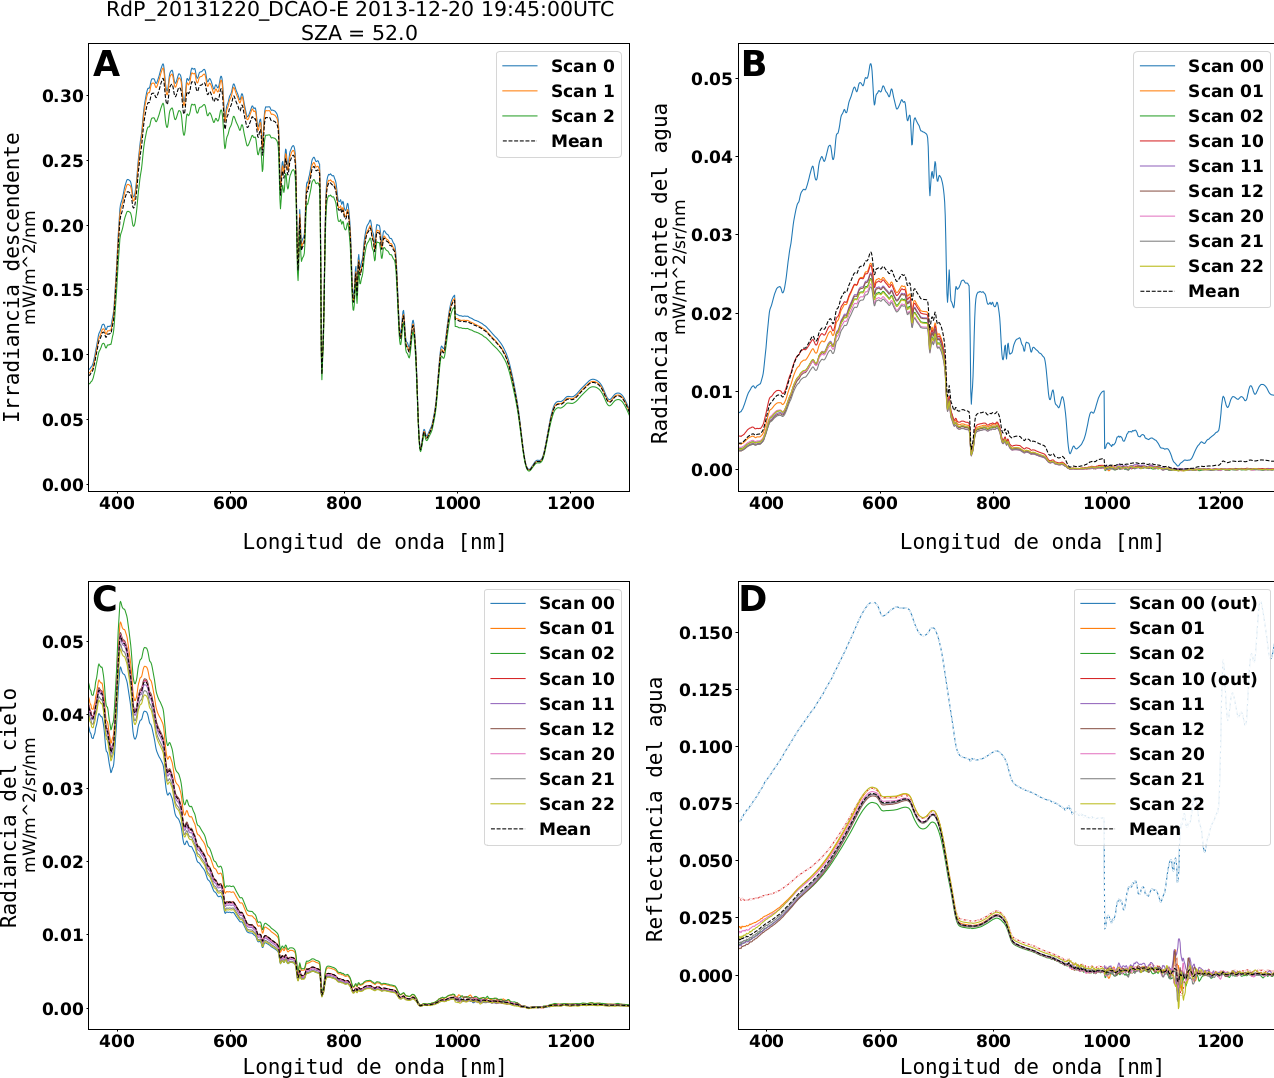
\includegraphics[width=\textwidth]{dat/figures/ASD_QC.png}
            \caption[Control de calidad de los escaneos hechos con el ASD para la estación RdP\_20131220\_DCAO-E.]{Control de calidad de los escaneos hechos con el ASD para la estación RdP\_20131220\_DCAO-E. a) Escaneos de irradiancia descendente, $E_{d}$. b) Escaneos de radiancia ascendente, $L_{u}$. c) Escaneos de radiancia del cielo, $L_{sky}$. d) Reflectancia del agua, $\rho_{w}$, para cada una de las nueve series. Obsérvese que la media computada no tiene en cuenta los espectros anómalos 00 (proveniente de una mala medición de $L_{u}$) y 10 (subestimación de la componente especular del cielo).} 
            \label{dat:ASD_QC}
            \end{figure}


    \subsection{Sistema radiométrico TriOS}
    \label{dat:s:trios}
        
        El radiómetro TriOS mide la luz reflejada en la región visible/infrarrojo cercano (VNIR, $350-950$ nm). A pesar de no medir en el rango del SWIR (en que sí mide el ASD), tiene la ventaja de que mide en simúltaneo los tres espectros requeridos ($E_{d}$, $L_{u}$ y $L_{sky}$), dado que el equipo consta de dos radiómetros y un irradiómetro. Esto lo hace mucho más fácil de operar, y una vez colocado en un soporte mecánico, será mucho más fácil garantizar el correcto posicionamiento de los sensores que en el caso de ASD.

        \subsubsection{TriOS: Protocolo de medición}
        \label{dat:s:triosMed}

            \begin{figure}
            \centering
            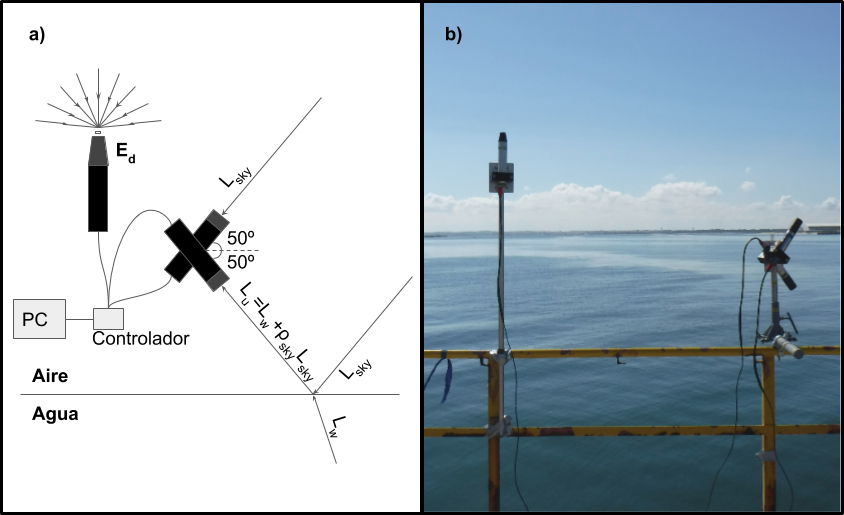
\includegraphics[width=\textwidth]{dat/figures/TriOS.png}
            \caption[Disposición del radiómetro TriOS utilizada para las mediciones.]{Disposición del radiómetro TriOS utilizada para las mediciones. Los tres sensores se manipulan desde el mismo controlador, lo que garantiza simultaneidad de los escaneos. a) Esquema de la geometría (cenital) indicada para los radiómetros ($L_{u}$ y $L_{sky}$) y el irradiómetro ($E_{d}$). b) Fotografía del sistema TriOS colocado sobre el Muelle de Barreiro, en la costa del Estuario del Río Tajo, en Lisboa, Portugal (campaña Tagus\_20190617).}
            \label{dat:TriOS}
            \end{figure}

            El protocolo de medición de TriOS es mucho más sencillo que el del ASD, dado que las mediciones son controladas por un \textit{software} (MSDA\_XE) que automáticamente computa los tiempos de integración y envía las órdenes a los tres sensores para que ejecuten las mediciones en dichos tiempos. Una vez que se quiere realizar la medición, se acciona un disparador global, el cual se mantendrá activo durante aproximadamente 15 minutos. Se fijó esta ventana temporal ya que es lo suficientemente grande como para abarcar una cantidad adecuada de mediciones que superen los estándares de calidad y suficientemente chica como para evitar efectos de varibilidad natural sobre la medición final reportada.
    
        \subsubsection{TriOS: Protocolo de procesamiento}
        \label{dat:s:triosProc}
            
            Los criterios de control de los escaneos se enumeran a continuación:

            \begin{enumerate}
                \item \textbf{Sincronicidad de escaneos}: Seleccionamos previamente los escaneos $E_{d}$, $L_{u}$ y $L_{sky}$ que se sincronizan mutuamente (por ejemplo, eliminamos los escaneos $E_{d}$ que no son simultáneos con ninguno de los de $L_{sky}$ o $L_{u}$). Esto puede suceder cuando los tiempos de integración de los sensores (optimizados automáticamente por TriOS) difieren entre sí. Esto podría ser causado, por ej., por una sombra incidental en cualquiera de los sensores durante las mediciones.

                \item \textbf{Anomalías espectrales}: Descartamos los escaneos que presentan saltos discontinuos (no físicos) en rangos espectrales muy cortos. Hacemos esto comparando valores medidos por el TriOS en longitudes de onda consecutivas. Más precisamente, el escaneo pasa dicho control de calidad si todas las magnitudes $M$ (siendo $E_{d}$, $L_{sky}$ o $L_{sea}$) satisface:
            
                \begin{equation}
                \begin{aligned}
                    M[t_{0}; \lambda + 2.5] - M[t_{0}; \lambda] & <  \alpha[M]*(M[t_{0}; \lambda + 2.5] + M[t_{0}; \lambda])/2\\
                    \alpha[M = E_{d}  ] & = 0.4\\
                    \alpha[M = L_{se} ] & = 2.0\\
                    \alpha[M = L_{sky}] & = 0.4                      
                \end{aligned}
                \end{equation}
                
                Esto se verifica para todos los tiempos de exploración $t_{0}$ y debe cumplirse para todas las longitudes de onda en $[400-947.5]$ nm.

                \item \textbf{Anomalías temporales}: Descartamos los escaneos que presentan picos temporales repentinos. Hacemos esto comparando cada escaneo a tiempo $t=t_{0}$ con el escaneo anterior/posterior, a $t_{0}\pm dt$ a la longitud de onda particular de $550$ nm. Más precisamente, el escaneo deberá satisfacer:

                \begin{equation}
                \begin{aligned}
                    M[t_{0} \pm dt; 550] - M[t_{0}; 550] & <  \beta[M]*(M[t_{0} \pm dt; 550] + M[t_{0}; 550])/2\\
                    \beta[M = Ed  ] & = 0.25\\
                    \beta[M = Lse ] & = 0.25\\
                    \beta[M = Lsky] & = 0.25\\
                \end{aligned}
                \end{equation}
            
                \item \textbf{Desvío de $E_{d}$ del cenit}: Descartamos aquellos escaneos donde el ángulo comprendido entre la medición de $E_{d}$ y el cenit (medido con un inclinómetro adosado al irradiómetro) es mayor a $5 \degree$.
            
                \item \textbf{Selección de escaneos y cómputo de estadísticos}: Una vez que todos estos criterios son considerados, seleccionamos los primeros 5 escaneos válidos (i.e. que hayan pasado todos los controles anteriores). Para este conjunto de escaneos se computan la media ($\mu$), el desvío estándar ($\sigma$) y el coeficiente de variación ($CV = 100\times\sigma/\mu$).

                La Figura \ref{dat:TriOS_QC} muestra cómo dichos criterios fueron aplicados a los escaneos de la estación RdP\_20181202\_ST05.
            
                \begin{figure}
                \centering
                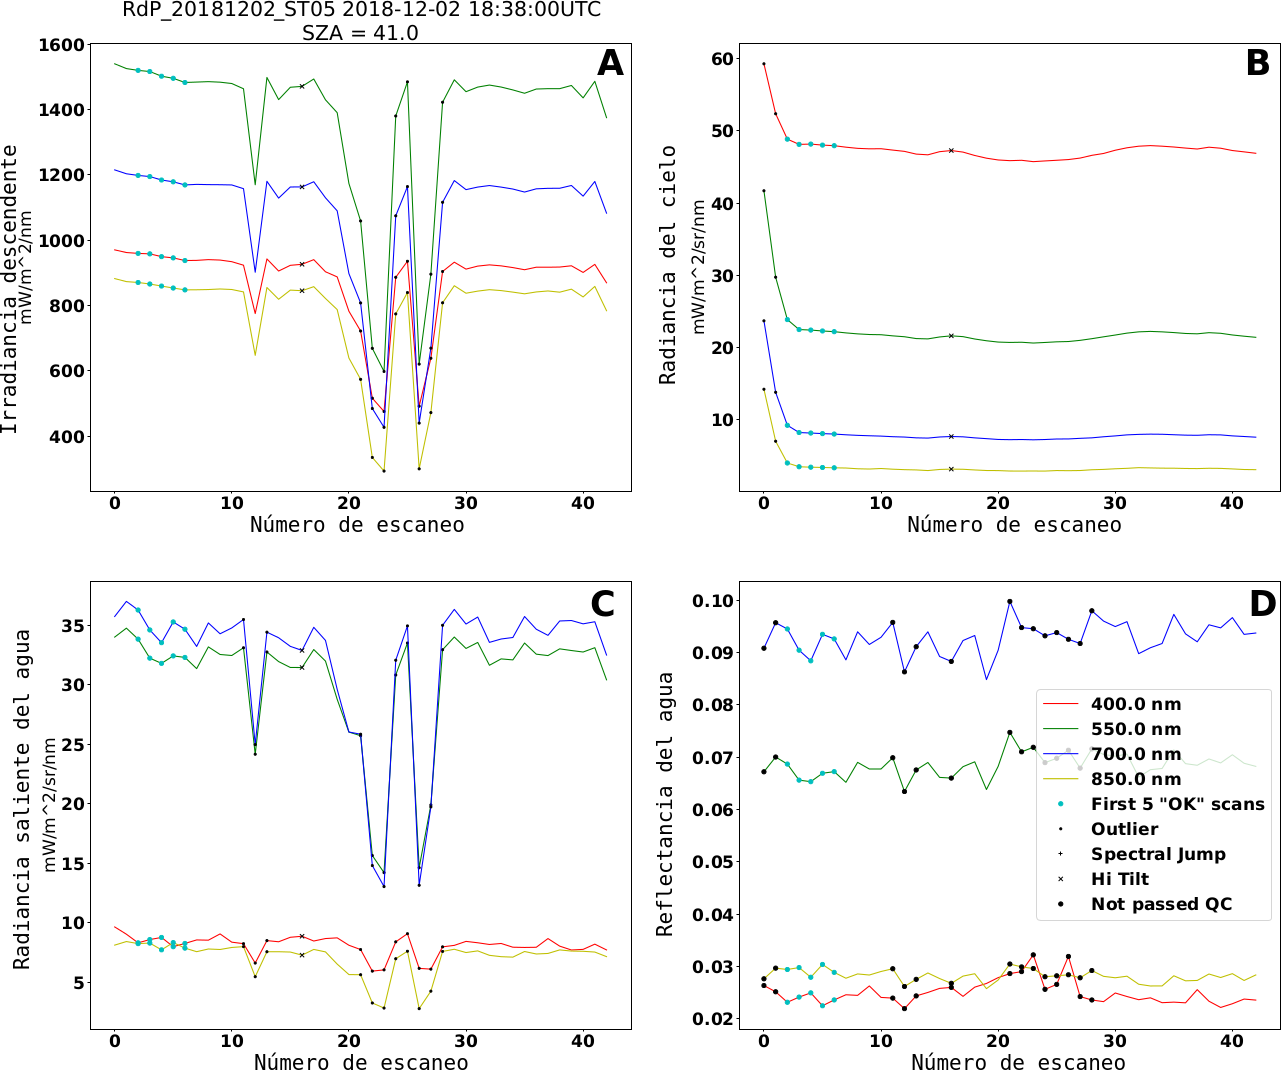
\includegraphics[width=\textwidth]{dat/figures/TriOS_QC.png}
                \caption[Control de calidad de los escaneos hechos con el TriOS para la estación RdP\_20181202\_ST05.]{Control de calidad de los escaneos hechos con el TriOS para la estación RdP\_20181202\_ST05. Escaneos a 400 nm, 550 nm, 700 nm y 850 nm de irradiancia descendente, $E_{d}$ (a), radiancia ascendente, $L_{u}$ (b), radiancia del cielo, $L_{sky}$ (c) y reflectancia del agua, $\rho_{w}$ (d). Todos los criterios de calidad mencionados previamente (anomalías temorales, espectrales y de ángulo cenital elevado) son evaluados previo a seleccionar los primeros cinco escaneos de calidad (señalados en cian).} 
                \label{dat:TriOS_QC}
                \end{figure}
                
                
                \item \textbf{Condiciones de baja variabilidad}: La siguiente condición debe ser satisfecha para asegurar una variabilidad aceptablemente baja entre los 5 escaneos seleccionados:
                
                \begin{equation}
                    std(\rho_{w}(750)) < 0.05
                \end{equation}
            \end{enumerate}
            
\section{Mediciones de turbidez}
\label{dat:s:turbidez}

    La \textit{turbidez} puede ser definida cualitativamente como la reducción de la transparencia de un líquido causada por la presencia de materia no disuelta.
    En términos ópticos, y siguiendo el estándar definido por la norma ISO 7027, la turbidez de una muestra de fluido (en nuestro caso, aguas naturales) se establece determinando qué fracción de luz - proveniente de un LED en el inrarrojo cercano - es dispersada a $90\degree$ por una muestra dada. A su vez, se puede refinar la medición determinando en simultáneo la fracción transmitida del haz incidente. Un instrumento que mide la turbidez únicamente a partir de la dispersión a $90\degree$ se denomina \textit{nefelómetro}; mientras que si se vale a su vez de la detección de la fracción de radiación transmitida el instrumento se denomina \textit{turbidímetro}. Los fotones capturados por el/los fotodiodo/s se transforman en una corriente eléctrica que es trasducida a unidades de turbidez. Si el nefelómetro o turbidímetro es calibrado según los estándares de la ISO 7027, las unidades utilizadas se llaman FNU (Formazin Nephelometric Units). Estas unidades se refieren a una sustancia patrón llamada formazina y se convierten idénticamente a la concentración de dicha sustancia en \textit{mg/l}. Es decir que se trasduce al valor de \textit{x FNU} al voltaje medido por el nefelómetro/turbidímetro sobre una muestra de formazina (en agua pura) de concentración \textit{x mg/l}.
    
    Existen diversas unidades de medición de turbidez según la sustancia patrón utilizada, la fuente emisora y la geometría de detección de los fotodiodos del sensor. En este capítulo utilizaremos dos unidades, ambas determinadas a partir de la formazina: las FNU (ya descritas) y las FBU (\textit{Formazin Backscatter Units}). Tal como su nombre lo indica, estas útlimas corresponden a la trasducción voltaje-concentración de formazina, pero utilizando un retrodispersómetro en vez de un nefelómetro. Es fundamental notar que, for definición, dichas unidades son equivalentes \textit{para una muestra de formazina}, es decir, \textit{1 FNU = 1 FBU = 1 mg/l} de formazina. Sin embargo, dicha identidad no es válida en el caso general, sino que la relación entre estas unidades será dependiente de la geometría de la función de dispersión volumétrica (\textit{Volume Scattering Function}, VSF o $\beta$, Ec. \ref{qssa:eq:vsf}) de la muestra considerada.
    
    Hay un gran interés de los usuarios en monitorear la turbidez de las aguas costeras y estuarinas (Dogliotti et al. 2015, \cite{dogliotti2015}). El mapeo satelital de la turbidez es relevante tanto como un indicador del entorno óptico para fines de monitoreo de la calidad del agua (Nechad et al. 2009, \cite{nechad2010}) como por ser un \textit{proxy} fácilmente medible de la concentración de partículas suspendidas (SPM) en aplicaciones de transporte de sedimentos (Gippel 1995, \cite{gippel1995}). Con respecto al monitoreo de la calidad del agua, la turbidez es considerada un parámetro obligatorio que deben medir los estados miembros de la Unión Europea en la Directiva Marco de la Estrategia Marina (Unión Europea, 2008, \cite{eu2008}).

    \subsection{Turbidímetro portátil \textit{HACH 2100Q is}}
    \label{dat:s:hach}

        El \textit{HACH 2100Q is} es un turbidímetro portátil que satisface el estándar de la ISO 7027. Este instrumento determina la turbidez mediante la razón de la radiación dispersiada a $90 \degree$ y la transmisitida, proveniente de un LED a 860 nm (Figura \ref{dat:HACH}). El instrumento mide turbidez entre 0 y 999 FNU con una resolución de tres dígitos y fue programado para promediar una serie de 12 escaneos sucesivos para minimizar el impacto del ruido.
        
        \begin{figure}
        \centering
        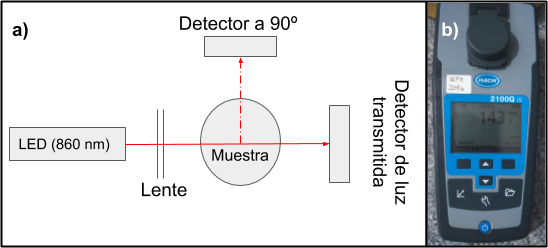
\includegraphics[width=0.8\textwidth]{dat/figures/HACH.png}
        \caption[Esquema y fotografía del turbidímetro portátil \textit{HACH 2100Q is} (ISO 7027).]{Turbidímetro portátil \textit{HACH 2100Q is} (ISO 7027). a) Esquema del funcionamiento del turbidímetro. b) Fotografía de uno de los turbidímetros utilizados en nuestro grupo (IAFE 2016), reportando un valor de 143 FNU (tras haber promediado 12 escaneos).}
        \label{dat:HACH}
        \end{figure}

        \subsubsection{HACH: Protocolo de medición}
        \label{dat:s:hachMed}

            Para realizar las mediciones se utiliza la siguiente metodología:
            \begin{itemize}
                \item Chequear la estabilidad del instrumento usando los estándares de formazina.
                \item Enjuagar y llenar el vial de vidrio con la muestra (10 ml).
                \item Enjuagar el lado exterior del vial con agua ultra pura (milliQ).
                \item Secar el exterior con papel de pulpa de celulosa (tisú).
                \item Ungir la cara exterior del vial con gel de silicona para homogeneizar el índice de refracción del vial en caso de que el vidrio presentase microgrietas de vidrio.
                \item Voltear suavemente la muestra para homogeneizarla. Evitar la formación de burbujas y gotas de condensación que pudieren alterar la medición.
                \item Realizar la medición de turbidez con el HACH 3 veces repitiendo el paso anterior entre cada repetición.
            \end{itemize}
            A partir de estas tres mediciones se obtendrán el valor medio y el desvío estándar y se asociarán al valor reportado con su error, respectivamente.

        \subsubsection{HACH: Protocolo de procesamiento}
        \label{dat:s:hachProc}
        
            El único control de calidad que se hace sobre las mediciones una vez realizadas es chequear que el coeficiente de variación no supere el 20 \%. En caso de superarse, se descarta la medición más alejada de la mediana. De todas formas, esta situación es extremadamente rara - de hecho, jamás se nos presentó - dado que el turbidímetro HACH provee mediciones muy estables que suelen tener coeficientes de variación menores al 5\%.
    
    \subsection{Medidores de turbidez en continuo \textit{OBS501}}
    \label{dat:s:obs}
    
    % , por lo que los llamaremos turbidímetros al igual que el HACH, aunque no satisfacen propiamente la definición planteada en la \S \ref{dat:s:turbidez}
        El sensor OBS501 es una combinación de dos dispersómetros (calibrados en unidades de turbidez) de medición continua que, al contrario del HACH, mide estando sumergido en el agua (Figura \ref{dat:OBS}). Ambos medidores de turbidez sensan la luz emitida por un láser VCCS (Voltage-Controlled Current Source) a 850 nm: uno de ellos es un nefelómetro (ISO 7027) y el otro un \textit{retrodispersómetro}. Ambos fueron calibrados con formazina, por lo que el nefelómetro provee valores de turbidez en FNU (magnitud llamada aquí T\_OBS501\_SS, por \textit{side-scattering}), mientras que el retrodispersómetro provee valores en FBU (magnitud llamada aquí T\_OBS501\_BS, por \textit{back-scattering}). Es importante notar que, a diferencia del HACH, el OBS carece de transmisómetro.
        
        \begin{figure}
        \centering
        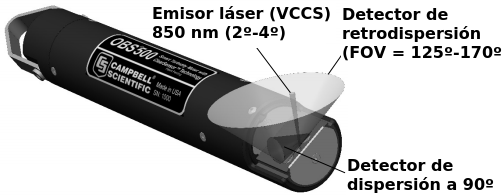
\includegraphics[width=0.8\textwidth]{dat/figures/OBS.png}
        \caption[Fotografía del OBS mostrando los conos de emisión del láser y sensado del nefelómetro y el retrodispersómetro.]{Fotografía del OBS mostrando los conos de emisión del láser y sensado del nefelómetro (T\_OBS501\_SS) y el retrodispersómetro (T\_OBS501\_BS).}
        \label{dat:OBS}
        \end{figure}

        \subsubsection{OBS: Protocolo de medición}
        \label{dat:s:obsMed}

            El OBS501 mide sumergido en el cuerpo de agua, aunque su autonomía es limitada, dado que debe ser comandado desde la superficie por un controlador (o \textit{datalogger}) no sumergible, el \textit{CR-800}. El CR-800 envía diversos comandos  - escaneo, encendido, apagado y activación del limpia-ópticas - al OBS 501 establecidos en un programa escrito en \textit{CRBasic}. En nuestro caso, se diseñó un programa que permitió ejecutar el siguiente protocolo: durante cada jornada de medición, el OBS501 se dispuso a medir cada 5 segundos durante un período continuo que abarcó desde la primera hasta la última de las estaciones de la jornada en determinado sitio.% Luego, se establecieron una serie de criterios para determinar el valor e incerteza de cada estación, detallados en la próxima sección.
            
        
        \subsubsection{OBS: Protocolo de procesamiento}
        \label{dat:s:obsProc}
        
            Para cada campaña se obtienen los valores en continuo de todas los datos de turbidez en FNU (T\_OBS501\_SS) y FBU (T\_OBS501\_BS), entre otras variables misceláneas. Estos datos se almacenan según tres criterios temporales: los datos en crudo, los datos suavizados a 1 minuto y los datos por estación.
            
            Tanto para los datos suavizados como para los datos por estación se selecciona una ventana temporal de los datos crudos: en el primer caso, una ventana móvil de 1 minuto y en el segundo, una ventana de 5 minutos centrada en el horario oficial de la estación (determinado generalmente por la medición radiométrica). En ambos casos, se eliminan escaneos anómalos dentro de dicha ventana, apelando al criterio del rango intercuartil (\textit{Inter-Quartile Range}, IQR, similar a Ec. \ref{dat:eq:ITR}), es decir, \textit{x} es un escaneo anómalo si:
            
            \begin{equation}
                \begin{aligned}
                x &> Q3 + 1.5 IQR\\
                x &< Q1 - 1.5 IQR
                \end{aligned}    
                \label{dat:eq:IQR}
            \end{equation}

            \noindent 
            siendo \textit{Q1} y \textit{Q3} los primer y tercer cuartiles. Una vez eliminados los valores anómalos, se computan la mediana y el desvío estándar dentro de la ventana y se asocian al valor reportado y a la incerteza, respectivamente. Si el coeficiente de variación supera el 15\%, el valor de la ventana no es considerado de buena calidad.

    \subsection{Validación del algoritmo de turbidez de Dogliotti et al. 2015}
    \label{dat:s:dog15}

        A su vez, para intercomparar las mediciones de turbidez con las radiométricas se computó y testeó el algoritmo de turbidez propuesto por Dogliotti et al. 2015, \cite{dogliotti2015} a partir de las reflectancias del agua medidas:

        \begin{equation}
        \begin{aligned}
            T(\lambda) & = \frac{A(\lambda).\rho_{w}(\lambda)}{1-\rho_{w}(\lambda)/C(\lambda)}, \quad\quad \lambda = 645\,nm,\,860\,nm\\
            \omega & = max\{min\{(\rho_{w}(645)-0.05)/0.02;1\};0\}\\
            T\_Dogliotti & = T(645).(1-\omega) + T(860).\omega
        \end{aligned}
        \label{dat:eq:dogliotti2015}
        \end{equation}

        \noindent siendo $A(645) = 228.1$ FNU, $A(860) = 3078.9$ FNU, $C(645) = 0.1641$ y $C(860) = 0.2112$.

\section{Mediciones de Material Particulado en Suspensión}
\label{dat:s:spm}

    La concentración de material particulado total en suspensión (\textit{Suspended Particulate Matter}, SPM) es la razón entre la masa neta del material colectado en un filtro GF/F por filtración y el correspondiente volumen de agua filtrado. Es una concentración masa en volumen y sus unidades usuales son $mg/l$. El método utilizado se denomina \textit{gravimétrico} y está descripto en Tilstone et al. 2003, \cite{tilstone2003} y basado en van der Linde 1998, \cite{vanderlinde1998}.
    
    \subsection{SPM: Protocolo de medición}
    \label{dat:s:spmMed}

        Las muestras de superficie son filtradas en filtros GF/F pre-combustionados y pre-pesados y luego de filtrar la muestra (Figura \ref{dat:SPM}), los mismos son secados y vueltos a pesar, para obtener así el peso por unidad de volumen filtrado. La concentración del material particulado inorgánico (SIM, \textit{Suspended Inorganic Matter}) se calcula mediante el combustionado posterior de los filtros, para eliminar los compuestos orgánicos, y repesado de los mismos. Finalmente la concentración del material particulado orgánico (SOM, \textit{Suspended Organic Matter}) se estima a partir de la diferencia entre el inorgánico y el total. La metodología es descrita a continuación:
        
        \begin{itemize}
            \item Preparación de los filtros
            \begin{itemize}
                \item Pre-combustión de los filtros a 450$\degree$C por 1 hora y lavado con agua milliQ.
                \item Secado de los filtros a 75$\degree$ C por 1 hora y almacenamiento en gel de silicona.
            \end{itemize}
            \item Determinación de SPM
                \begin{itemize}
                    \item Pesaje de los filtros secos (pesaje \textit{M0}).
                    \item Filtrado de un volumen de muestra (\textit{V}) a presiones de succión de $300-400 mmHg$.
                    \item Secado de los filtros en estufa a 75$\degree$C por 24 horas.
                    \item Pesaje de los filtros en la misma balanza usada previamente (pesaje \textit{M1}).
                    \item Determinación de SPM a partir de:
                        \begin{equation}
                            SPM = (M1-M0)/V
                            \label{dat:eq:SPM}
                        \end{equation}
                \end{itemize}
            \item Determinación de SIM y SOM
                \begin{itemize}
                    \item Combustionado de los filtros a 450$\degree$C por 5 horas (ó 4 horas a 550$\degree$C)
                    \item Pesaje de los filtros en la misma balanza usada previamente (pesaje \textit{M2})
                \end{itemize}
                \item Determinación de SIM y SOM a partir de:
                \begin{align}
                    SIM & = (M2-M0)/V\\
                    SOM & = SPM-SIM
                \end{align}
        \end{itemize}

        \begin{figure}
            \centering
            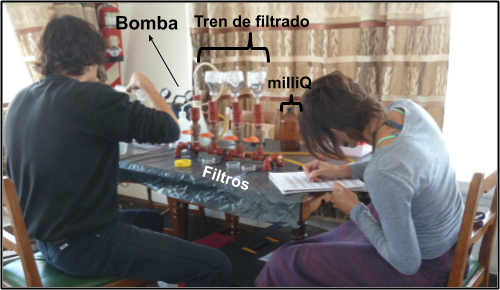
\includegraphics[width=0.75\textwidth]{dat/figures/SPM.png}
            \caption[Fotografía del tren de filtrado utilizado para obtener las mediciones de material particulado total, inorgánico y orgánico.]{Fotografía del tren de filtrado generalmente utilizado para obtener las mediciones de material particulado total (SPM), inorgánico (SIM) y orgánico (SOM).}
            \label{dat:SPM}
        \end{figure}
            
    \subsection{SPM: Protocolo de procesamiento}
    \label{dat:s:spmProc}
    
        Las mediciones por estación suelen hacerse por triplicado (de lo contrario se utiliza un único filtro). En dicho caso, se toma como valor reportado e incerteza a la media y desvío estándar y se descarta la medición si el coeficiente de variación supera el 20\%. 

    \subsection{Validación del algoritmo de SPM de Nechad et al. 2010}
    \label{dat:s:spmNech10}

        Por último, para comparar las mediciones de SPM con las radiométricas se computó y testeó el algoritmo de SPM propuesto por Nechad et al. 2010, \cite{nechad2010}, a partir de las reflectancias del agua medidas:

        \begin{equation}
            SPM\_Nechad = \frac{A(645).\rho_{w}(645)}{1-\rho_{w}(645)/C(645)} + B(645)
            \label{dat:eq:nechad2010}
        \end{equation}

        \noindent
        siendo $A(645) = 253.51 mg/l$, $B(645) = 2.32 mg/l$ y $C(645) = 0.1641$.
        
        
\section{Estructura de la base de datos}
\label{dat:s:basedatos}
    La base de datos presentada en este capítulo se creó siguiendo la lógica estándar de organización de la información usada en lenguajes de consulta de datos (DQLs, \textit{data query languages}, ver Cuadro \ref{dat:tab:metadata}). Es decir, los datos se estructuran en tablas bidimensionales en que cada columna se corresponde con un campo (por ejemplo, la latitud) y cada nueva fila una nueva entrada a la base de datos - una estación. A su vez, cada entrada/estación posee un código único identificatorio llamado \textit{llave} (\textit{key} en DQLs) que permite concatenar con sencillez los campos correspondientes a distintas tablas, y que debe figurar en todas ellas. A modo de ejemplo, supongamos que queremos comparar los datos de turbidez y los de SPM, cuyos campos se hallan en distintas tablas. El hecho de que en ambas figure el campo llave nos permite concatenarlas evitando errores que puedan surgir de la ausencia de entrada para alguna estación en alguno de los campos requeridos. 
    
    \subsection{Sistematización de las diferentes entradas}
    \label{dat:s:entradas}

        Los datos iniciales que conforman la base de datos no estaban originalmente estructurados siguiendo la lógica DQL, por lo que fue necesario reorganizarlos para poder generar un formato común de almacenamiento. De esta forma, se estructuraron las entradas (estaciones) de la base según a qué región pertenecían y según la campaña en la que fueron realizadas. Para cada región se asignó una sigla o acrónimo (e.g. \textit{RdP} para el Río de la Plata, \textit{BALakes} para las lagunas de la Provincia de Buenos Aires) y para nombrar a cada campaña se yuxtapuso a dicha sigla la fecha de la jornada inicial en formato $aaaammdd$ (año-mes-día). Por ejemplo, el Cuadro \ref{dat:tab:metadata} corresponde a la campaña $RdP\_20180404$, es decir, realizada en algún sitio del RdP a partir del 4 de abril de 2018.
        
        Para cada campaña se generó un subdirectorio dentro del directorio de la región correspondiente donde se archivaron las entradas en varias hojas de formato Excel, cada cual conteniendo un conjunto determinado de campos. Por ejemplo, el Cuadro \ref{dat:tab:metadata} corresponde a la hoja de Excel \textit{StationInfo}, donde se guardan los campos de la informacion general de las estaciones: horario de inicio y finalización, fecha, día, latitud, longitud, pasadas satelitales, etc.
                    
    \subsection{Código indentificatorio único de cada estación}
    \label{dat:s:codigo}
     
        Originalmente, la base de datos no poseía un campo al que se le pudiera asignar el rol de llave o código identificatorio. Si bien, dentro de cada campaña, cada estación se nombró de manera unívoca, entre campañas existían entradas de llave repetida que no necesariamente correspondían a la misma ubicación geográfica ni fecha. Para solventar esto se yuxtapuso del nombre de la campaña al nombre de la estación para generar la llave. Por ejemplo, la llave \textit{RdP\_20130430\_PP02-04} corresponde unívocamente a la estación PP02-04 de la campaña realizada a partir del 30 de abril del 2013 en la región del RdP.
        
        La razón por la que se dividieron los datos a partir de las distintas regiones y campañas y los distintos campos en planillas Excel y no en un gran archivo que contuviera a todos los datos fue fundamentalmente la de facilitar la visualización e interpretación de los mismos por los usuarios y garantizar la estabilidad del \textit{software} utilizado para hacer las consultas a la base. Dicho \textit{software} es el módulo \textit{pandas} (Python Data Analysis Library) del lenguaje de programación \textit{Python}. Aparte, los datos recopilados previo al inicio de la construcción de la base fueron históricamente jerarquizados según región y campaña, por lo que se prefirió sostener la jerarquización preexistente.
    
        \begin{table}
        \tiny
        \caption{Información general de las estaciones correspondientes a la campaña RdP\_20180404}
        \begin{adjustbox}{angle=90}
        \begin{tabularx}{1.4\textwidth}{|l|l|l|X|X|X|X|X|X|X|X|X|}
        \hline
        \rowcolor[HTML]{FFFC9E} 
        \textbf{Station ID} & \textbf{Region} & \textbf{Subregion} & \textbf{Pontoon/Vessel/Place} & \textbf{Lat} & \textbf{Lon} & \textbf{Date UTC} & \textbf{start Time UTC} & \textbf{end Time UTC} & \textbf{time Stamp UTC} & \textbf{Overpasses} \\ \hline
        P01 & RdP & CABA & Palermo (Pier) & -34.560754 & -58.39881 & 04/04/18 & 13:36 & 13:46 & 04/04/2018 13:36:00 &  \\ \hline
        P02 & RdP & CABA & Palermo (Pier) & -34.560754 & -58.39881 & 04/04/18 & 14:04 & 14:14 & 04/04/2018 14:04:00 & S2B \\ \hline
        P03 & RdP & CABA & Palermo (Pier) & -34.560754 & -58.39881 & 04/04/18 & 14:34 & 14:49 & 04/04/2018 14:34:00 &  \\ \hline
        P04 & RdP & CABA & Palermo (Pier) & -34.560754 & -58.39881 & 04/04/18 & 15:04 & 15:14 & 04/04/2018 15:04:00 &  \\ \hline
        P05 & RdP & CABA & Palermo (Pier) & -34.560754 & -58.39881 & 04/04/18 & 16:04 & 16:16 & 04/04/2018 16:04:00 &  \\ \hline
        P06 & RdP & CABA & Palermo (Pier) & -34.560754 & -58.39881 & 04/04/18 & 17:20 & 17:25 & 04/04/2018 17:20:00 &  \\ \hline
        P07 & RdP & CABA & Palermo (Pier) & -34.560754 & -58.39881 & 04/04/18 & 17:30 & 17:45 & 04/04/2018 17:30:00 & VIIRS \\ \hline
        P08 & RdP & CABA & Palermo (Pier) & -34.560754 & -58.39881 & 04/04/18 & 18:32 & 18:44 & 04/04/2018 18:32:00 &  \\ \hline
        P09 & RdP & CABA & Palermo (Pier) & -34.560754 & -58.39881 & 05/04/18 & 13:00 & 13:10 & 04/05/2018 13:00:00 &  \\ \hline
        P10 & RdP & CABA & Palermo (Pier) & -34.560754 & -58.39881 & 05/04/18 & 13:43 & 14:01 & 04/05/2018 13:43:00 & S3A \\ \hline
        P11 & RdP & CABA & Palermo (Pier) & -34.560754 & -58.39881 & 05/04/18 & 14:35 & 14:49 & 04/05/2018 14:35:00 &  \\ \hline
        P12 & RdP & CABA & Palermo (Pier) & -34.560754 & -58.39881 & 05/04/18 & 15:38 & 15:51 & 04/05/2018 15:38:00 &  \\ \hline
        P13 & RdP & CABA & Palermo (Pier) & -34.560754 & -58.39881 & 05/04/18 & 16:38 & 16:49 & 04/05/2018 16:38:00 &  \\ \hline
        P14 & RdP & CABA & Palermo (Pier) & -34.560754 & -58.39881 & 05/04/18 & 17:16 & 17:29 & 04/05/2018 17:16:00 & VIIRS \\ \hline
        P15 & RdP & CABA & Palermo (Pier) & -34.560754 & -58.39881 & 05/04/18 & 18:01 & 18:17:39 & 04/05/2018 18:01:30 & Aqua \\ \hline
        P16 & RdP & CABA & Palermo (Pier) & -34.560754 & -58.39881 & 05/04/18 & 18:40 & 18:50 & 04/05/2018 18:40:00 &  \\ \hline
        P17 & RdP & CABA & Palermo (Pier) & -34.560754 & -58.39881 & 06/04/18 & 13:33 &  & 04/06/2018 13:33:00 &  \\ \hline
        P18 & RdP & CABA & Palermo (Pier) & -34.560754 & -58.39881 & 06/04/18 & 14:38 &  & 04/06/2018 14:38:00 &  \\ \hline
        P19 & RdP & CABA & Palermo (Pier) & -34.560754 & -58.39881 & 06/04/18 & 15:33 &  & 04/06/2018 15:33:00 &  \\ \hline
        P20 & RdP & CABA & Palermo (Pier) & -34.560754 & -58.39881 & 06/04/18 & 16:38 &  & 04/06/2018 16:38:00 &  \\ \hline
        P21 & RdP & CABA & Palermo (Pier) & -34.560754 & -58.39881 & 06/04/18 & 17:39 &  & 04/06/2018 17:39:00 &  \\ \hline
        P22 & RdP & CABA & Palermo (Pier) & -34.560754 & -58.39881 & 06/04/18 & 18:41 &  & 04/06/2018 18:41:00 &  \\ \hline
        P-B & RdP & CABA & Palermo (Pier) & -34.562928 & -58.402581 & 06/04/18 & 19:00 &  & 04/06/2018 19:00:00 &  \\ \hline
        \end{tabularx}
        \end{adjustbox}
        \label{dat:tab:metadata}
        \end{table}

    \subsection{Sistematización de los diferentes campos}
    \label{dat:s:campos}

        Como ya fue mencionado, los campos se almacenaron en tablas diferentes según el instrumento de medición. A continuación, enumeramos algunos ejemplos:

        \begin{enumerate}
            \item \textbf{Radiometría}. Dado que los datos radiométricos son vectoriales, cada espectro obtenido se traduce en $N$ campos, siendo $N$ el número total de longitudes de onda ($N=241$ en el caso de TriOS, que fue dispuesto para medir en el rango $350:2.5:950$ nm; $N=2151$ en el caso de ASD, que fue dispuesto para medir en el rango $350:1:2500$ nm). Por lo que los productos espectrales finales derivados de la radiometría (reflectancia media y desvío estándar) son almacenados en hojas separadas para garantizar una visualización adecuada. A su vez, los productos intermedios derivados en el cómputo de estos espectros son guardados en planillas auxiliares (e.g. el conjuto total de escaneos, los valores medios de $E_{d}$, $L_{sky}$ y $L_{u}$, etc.). Por último, se guardan en una hoja aparte el coeficiente de Fresnel equivalente, $\rho_{sky}$, el ángulo cenital solar al momento de la adquisición, $SZA [\degree]$, y los campos de los estadísticos de relevancia a ser utilizados en los controles de calidad: $L_{sky}:E_{d}(750)$, $std[\rho_{w}(750)]$, $CV(780) [\%]$,	$CV(860) [\%]$ y $Max\{CV(400:900)\} [\%]$.	
            \item \textbf{Turbidez HACH}. Los datos de turbidez medidos con turbidímetros HACH se almacenaron según muestra el Cuadro \ref{dat:tab:hach}. Para ello fue necesario crear campos compuestos, dado que para cada turbidímetro HACH utilizado se guardan los triplicados, el promedio y el coeficiente de variación. El módulo \textit{pandas} permite identificar campos compuestos al indicarle un número de filas mayor a uno que corresponden a los nombres de los campos. En este caso, las primeras dos filas (en amarillo en el Cuadro \ref{dat:tab:hach} son interpretadas como descriptoras del campo correspondiente. Asimismo, \textit{pandas} almacena los campos compuestos como duplas de caracteres. Por ejemplo, al campo \textit{sample1} del turbidímetro \textit{HACH2016} se le asigna el nombre \textit{('HACH2016','sample1')}.
        \end{enumerate}

        \begin{table}
        \tiny
        \caption{Mediciones de turbidez (HACH) de las estaciones correspondientes a la campaña RdP\_20180404.}
        \begin{adjustbox}{angle=90}
        \begin{tabular}{|l|l|l|l|l|l|l|l|l|l|l|l|l|l|}
        \hline
        \rowcolor[HTML]{FFFC9E} 
        \cellcolor[HTML]{FFFC9E} & \cellcolor[HTML]{FFFC9E} & \cellcolor[HTML]{FFFC9E} & \cellcolor[HTML]{FFFC9E} & \multicolumn{5}{l|}{\cellcolor[HTML]{FFFC9E}\textbf{IAFE2016{[}FNU{]}}} & \multicolumn{5}{l|}{\cellcolor[HTML]{FFFC9E}\textbf{RBINS2009{[}FNU{]}}} \\ \cline{5-14} 
        \rowcolor[HTML]{FFFC9E} 
        \multirow{-2}{*}{\cellcolor[HTML]{FFFC9E}\textbf{\begin{tabular}[c]{@{}l@{}}Station\\ ID\end{tabular}}} & \multirow{-2}{*}{\cellcolor[HTML]{FFFC9E}\textbf{timeStampUTC}} & \multirow{-2}{*}{\cellcolor[HTML]{FFFC9E}\textbf{\begin{tabular}[c]{@{}l@{}}globalMean\\ {[}FNU{]}\end{tabular}}} & \multirow{-2}{*}{\cellcolor[HTML]{FFFC9E}\textbf{\begin{tabular}[c]{@{}l@{}}globalCV\\ {[}\%{]}\end{tabular}}} & \textbf{sample1} & \textbf{sample2} & \textbf{sample3} & \textbf{Mean} & \textbf{CV{[}\%{]}} & \textbf{sample1} & \textbf{sample2} & \textbf{sample3} & \textbf{Mean} & \textbf{CV{[}\%{]}} \\ \hline
        P01 & 04/04/2018 13:38:00 & 107.50 & 2.18 & 108.00 & 106.00 & 104.00 & 106.00 & 1.89 & 108.00 & 108.00 & 111.00 & 109.00 & 1.59 \\ \hline
        P02 & 04/04/2018 14:18:00 & 111.50 & 2.25 & 110.00 & 116.00 & 109.00 & 111.67 & 3.39 & 112.00 & 112.00 & 110.00 & 111.33 & 1.04 \\ \hline
        P03 & 04/04/2018 14:36:00 & 111.33 & 1.77 & 111.00 & 112.00 & 108.00 & 110.33 & 1.89 & 111.00 & 112.00 & 114.00 & 112.33 & 1.36 \\ \hline
        P04 & 04/04/2018 15:09:00 & 102.27 & 2.24 & 98.60 & 101.00 & 102.00 & 100.53 & 1.74 & 105.00 & 104.00 & 103.00 & 104.00 & 0.96 \\ \hline
        P05 & 04/04/2018 16:05:00 & 92.10 & 2.68 & 91.80 & 88.80 & 89.70 & 90.10 & 1.71 & 94.70 & 94.60 & 93.00 & 94.10 & 1.01 \\ \hline
        P06 & 04/04/2018 17:04:00 & 92.07 & 1.69 & 92.40 & 92.00 & 90.60 & 91.67 & 1.03 & 91.70 & 94.90 & 90.80 & 92.47 & 2.33 \\ \hline
        P07 & 04/04/2018 17:34:00 & 97.23 & 1.63 & 96.80 & 97.30 & 96.10 & 96.73 & 0.62 & 95.20 & 99.60 & 98.40 & 97.73 & 2.33 \\ \hline
        P08 & 04/04/2018 18:36:00 & 102.33 & 0.80 & 101.00 & 103.00 & 103.00 & 102.33 & 1.13 & 103.00 & 102.00 & 102.00 & 102.33 & 0.56 \\ \hline
        P09 & 04/05/2018 13:02:00 & 81.32 & 0.78 & 80.90 & 80.60 & 81.00 & 80.83 & 0.26 & 81.20 & 82.10 & 82.10 & 81.80 & 0.64 \\ \hline
        P10 & 04/05/2018 13:50:00 & 78.90 & 1.15 & 78.70 & 77.90 & 78.60 & 78.40 & 0.56 & 80.50 & 79.30 & 78.40 & 79.40 & 1.33 \\ \hline
        P11 & 04/05/2018 14:35:00 & 83.02 & 0.73 & 82.60 & 82.20 & 82.80 & 82.53 & 0.37 & 83.30 & 83.90 & 83.30 & 83.50 & 0.41 \\ \hline
        P12 & 04/05/2018 15:36:00 & 105.83 & 2.02 & 104.00 & 104.00 & 104.00 & 104.00 & 0.00 & 109.00 & 107.00 & 107.00 & 107.67 & 1.07 \\ \hline
        P13 & 04/05/2018 16:36:00 & 91.52 & 1.47 & 90.80 & 90.10 & 90.10 & 90.33 & 0.45 & 92.30 & 92.80 & 93.00 & 92.70 & 0.39 \\ \hline
        P14 & 04/05/2018 17:16:00 & 110.17 & 1.34 & 108.00 & 111.00 & 112.00 & 110.33 & 1.89 & 109.00 & 110.00 & 111.00 & 110.00 & 0.91 \\ \hline
        P15 & 04/05/2018 18:03:00 & 100.65 & 2.35 & 102.00 & 101.00 & 100.00 & 101.00 & 0.99 & 104.00 & 96.90 & 100.00 & 100.30 & 3.55 \\ \hline
        P16 & 04/05/2018 18:40:00 & 98.90 & 1.65 & 98.80 & 97.00 & 97.00 & 97.60 & 1.06 & 101.00 & 99.60 & 100.00 & 100.20 & 0.72 \\ \hline
        P17 & 04/06/2018 13:33:00 & 121.50 & 1.35 & 122.00 & 121.00 & 121.00 & 121.33 & 0.48 & 122.00 & 124.00 & 119.00 & 121.67 & 2.07 \\ \hline
        P18 & 04/06/2018 14:38:00 & 113.83 & 1.51 & 112.00 & 113.00 & 116.00 & 113.67 & 1.83 & 116.00 & 113.00 & 113.00 & 114.00 & 1.52 \\ \hline
        P19 & 04/06/2018 15:33:00 & 114.00 & 1.57 & 116.00 & 111.00 & 115.00 & 114.00 & 2.32 & 115.00 & 113.00 & 114.00 & 114.00 & 0.88 \\ \hline
        P20 & 04/06/2018 16:38:00 & 101.32 & 1.72 & 99.60 & 99.30 & 101.00 & 99.97 & 0.91 & 104.00 & 102.00 & 102.00 & 102.67 & 1.12 \\ \hline
        P21 & 04/06/2018 17:39:00 & 121.50 & 1.25 & 121.00 & 122.00 & 121.00 & 121.33 & 0.48 & 123.00 & 119.00 & 123.00 & 121.67 & 1.90 \\ \hline
        P22 & 04/06/2018 18:41:00 & 129.33 & 0.80 & 129.00 & 129.00 & 130.00 & 129.33 & 0.45 & 129.00 & 128.00 & 131.00 & 129.33 & 1.18 \\ \hline
        P-B &  &  &  &  &  &  &  &  &  &  &  &  &  \\ \hline
        \end{tabular}
        \end{adjustbox}
        \label{dat:tab:hach}
        \end{table}

\section{Resultados}
\label{dat:s:resultados}

    A continuación, exhibiremos los resultados del comportamiento global de las mediciones realizadas sobre las regiones consideradas (\S \ref{dat:s:areas}). Analizaremos primero las características espectrales de las mediciones radiométricas para cada región (\S \ref{dat:s:espectrales}) y luego intercompararemos los resultados obtenidos para las magnitudes no espectrales (turbidez y SPM, \S \ref{dat:s:noespectrales}).
    
    \subsection{Intercomparación de mediciones radiométricas}
    \label{dat:s:espectrales}
        
        En la Figura \ref{dat:HyperASD} se muestran todos los espectros obtenidos por el ASD para las campañas realizadas en el RdP. En dicha figura, cada espectro fue coloreado según su turbidez (obtenida al aplicar Ec. \ref{dat:eq:dogliotti2015}) siguiendo un mapa de colores logarítmico. A su vez, dicha figura exhibe la fuerte relación entre la forma espectral de las curvas obtenidas y la del coeficiente de absorción del agua líquida pura, \cite{pope1997}\cite{kou1993}. Dicha relación inversa (ascenso de la reflectancia con el descenso de la absorción y viceversa) es completamente compatible con lo esperado (véase Ec. \ref{qssa:eq:rhowmod0}). Se puede establecer que la peculiar \textit{similaridad} entre dichas curvas y la absorción del agua para longitudes de onda mayores a 700 nm (ya notada en Ruddick et al. 2006, \cite{ruddick2006}) se debe esencialmente: i) a que la variación espectral del coeficiente de retrodispersión de las partículas minerales presentes en el agua en este rango es suave (por lo que las variaciones de las reflectancias en rangos espectrales cortos son cuasi-independientes de la dispersión), y ii) al bajo coeficiente de absorción de biopigmentos en dicho rango combinado con las bajas concentraciones de fitoplancton en dichas aguas. Esto último se debe a la alta concentración de partículas minerales que implica a su vez un notable afinamiento de la capa eufótica, inhibiendo la presencia de organismos fotosintéticos. Se puede afirmar entonces que la curvatura de dichas reflectancias en el NIR/SWIR está casi enteramente dominada por la absorción del agua y su magnitud dominada por la concentración de sedimentos, lo cual se manifiesta en el hecho de que rara vez se observan \textit{intersecciones} entre dichas curvas, es decir, que siguen un orden secuencial a lo largo de todo este rango espectral.
        
        
        \begin{figure}
        \centering
        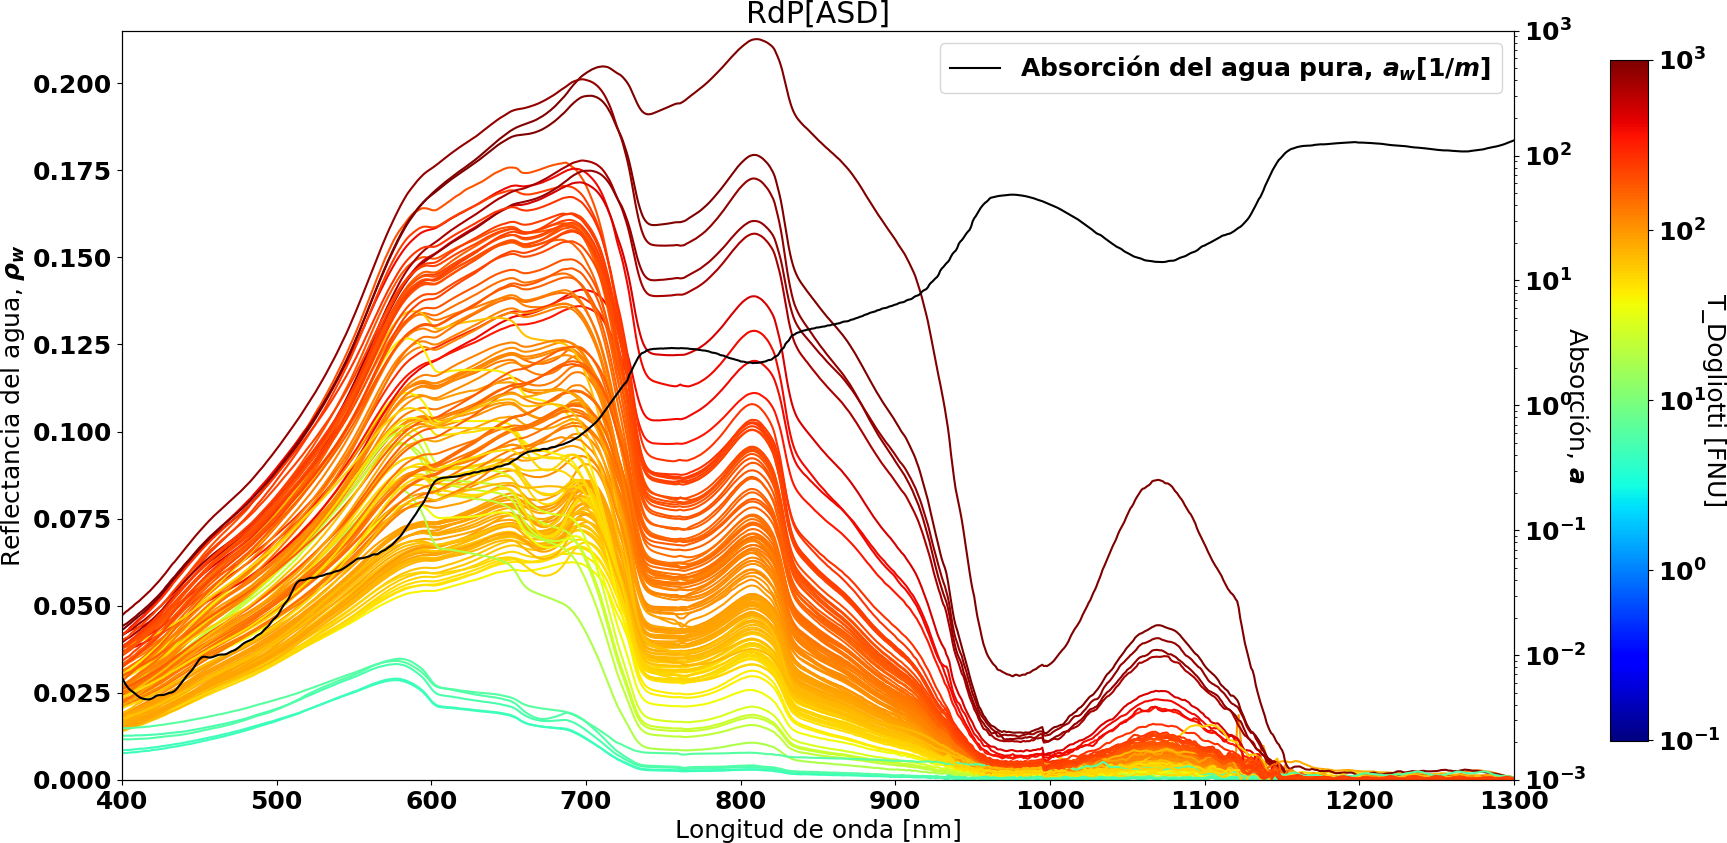
\includegraphics[width=\textwidth]{dat/figures/HyperASD.png}
        \caption[Reflectancias del agua obtenidas con el ASD sobre el RdP]{Reflectancias del agua obtenidas para todo el conjunto de campañas del RdP en que se midió con ASD (todas aquellas que pasaron el control de calidad). Las mismas están mapeadas a un mapa de colores escalado logarítmicamente con la turbidez de Dogliotti et al. 2015, \textit{T\_Dogliotti}. En negro, espectro de absorción del agua líquida pura, \cite{obpg}.}
        \label{dat:HyperASD}
        \end{figure}
    
        Por otro lado, si bien en el rango espectral de 500-700 nm también se observa una fuerte correlación entre las firmas medidas y la absorción del agua, las curvas comienzan a exhibir diferentes comportamientos que se distancian de la similaridad observada en el NIR/SWIR (se observa que las curvas frecuentemente se cortan entre sí). Esto es esperable dado que en este rango espectral el impacto de la eventual presencia de pigmentos y material orgánico coloreado disuelto (CDOM) es mayor y la dependencia espectral de la retrodispersión de partículas no algales más marcada que en el rango NIR/SWIR (véase Figura \ref{dat:HyperTriOS}).
        %
        Por último, en la región del utravioleta, violeta, azul y cian el impacto de la absorción del agua es difícilmente distinguible en las firmas espectrales, dado que entra a dominar en este rango la absorción de las partículas minerales y el CDOM, ambas marcadamente superiores que la del agua en este rango (\S \ref{qssa:s:iops_spm} y \ref{qssa:s:abs_cdom}).
        
        Otra cuestión a destacar de la Figura \ref{dat:HyperASD} es la presencia de firmas espectrales de muy baja turbidez ($\approx 3 FNU$) en comparación con los valores típicos observados en el RdP. Dichas firmas fueron obtenidas en la región de Samborombón (véase Figura \ref{dat:bardp}) en la zona de transición entre los regímen de aguas dulces y turbias de RdP y de aguas saladas del Océano Atlántico.
        También cercano a esta región se conforma el Frente de Turbidez (sobre la Barra del Indio, Framiñan y Brown 1996, \cite{framinan1996}), donde se presentan los valores más altos de turbidez/reflectancia medidos en el RdP (Figura \ref{int:rdp}).

        A partir de la Figura \ref{dat:HyperTriOS} (ídem Figura \ref{dat:HyperASD} pero para el sistema radiométrico TriOS) se pueden visibilizar las principales características distintivas de cada una de las regiones consideradas en el presente análisis. Las firmas del RdP no presentan diferencias sustanciales con las ya analizadas en la Figura \ref{dat:HyperASD}, excepto que en este caso el rango espectral abarcado se restringe a 400-900 nm. En esta figura, aparte del coeficiente de absorción del agua, se superpusieron los coeficientes de absorción específicos de partículas (\S \ref{qssa:s:iops_spm}), de la clorofila-a y la ficocianina, \cite{simis2012}, cuyos impactos son fuertemente observables en las firmas espectrales de Chascomús y en menor medida del Tajo, indicando una concentración más elevada de dichos pigmentos en comparación con el RdP. Nótese que la forma espectral de la absorción de la ficocianina es únicamente identificable en las firmas de Chascomús. Este pigmento es característico de las cianobacterias cuya presencia en esta laguna fue confirmada mediante el análisis al microscopio (\textit{com. pers}. Dra. Laura Sánchez, Laboratorio de Limnología EGE-IEGEBA, UBA/CONICET). Por el contrario, el pico de absorción de la clorofila-a en 680 nm (pigmento presente en todos las algas fotosintetizadoras) genera una depresión en las firmas espectrales de todas las regiones, si bien el efecto es marcadamente más pronunciado en las aguas de dicha laguna, donde la biomasa fitoplanctónica es mayor. A su vez, las aguas del Estuario del Tajo presentan firmas de valores más bajos, debido a concentraciones de SPM más bajas y un impacto fuerte de la clorofila-a. El impacto de la absorción de la ficocianina en las firmas de este estuario no es discernible del impacto de la absorción del agua líquida pura.
    
        \begin{figure}
        \centering
        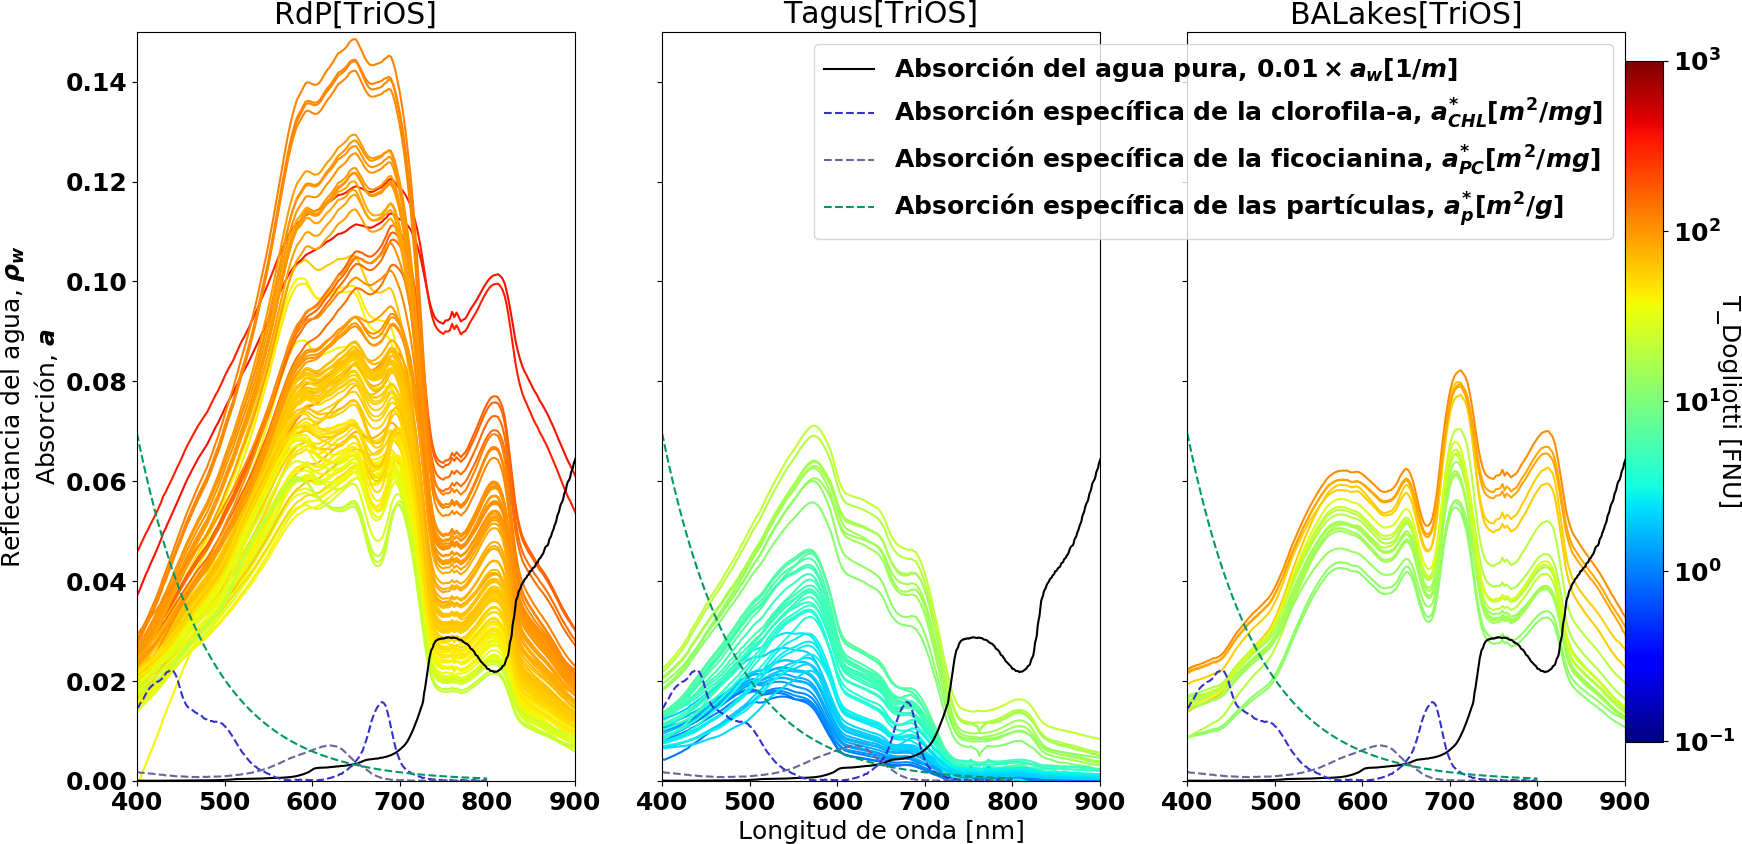
\includegraphics[width=\textwidth]{dat/figures/HyperTriOS.png}
        \caption[Reflectancias del agua medidas con el sistema radiométrico TriOS para las tres regiones consideradas: Río de la Plata, Estuario del Tajo y Laguna de Chascomús.]{Reflectancias del agua medidas con el sistema radiométrico TriOS para las tres regiones consideradas: Río de la Plata (RdP), Estuario del Tajo (Tagus) y Chascomús (BALakes). Se muestran a su vez espectros medios de absorción del agua líquida pura y absorciones específicas típicas de la clorofila-a (\S \ref{qssa:s:abs_pigmentos}), la ficocianina (\S \ref{qssa:s:abs_pigmentos}) y de partículas (\S \ref{qssa:s:iops_spm}).}
        \label{dat:HyperTriOS}
        \end{figure}

    \subsection{Intercomparación de mediciones no espectrales}
    \label{dat:s:noespectrales}
        
        Los rangos abarcados por cada una de las magnitudes no espectrales mencionadas en las secciones anteriores se visualizan en forma de diagramas de cajas en la Figura \ref{dat:boxplot}. En general, se observan valores más elevados de turbidez y SPM para el RdP y Chascomús en comparación con el Estuario del Tajo y un rango dinámico mayor en el RdP en comparación con las restantes. Esto último es esperable dado que el RdP abarca escenarios ópticos mucho más diversos que las otras regiones consideradas y aparte el número de estaciones realizadas excede ampliamente a los de las restantes regiones (véase Cuadro \ref{dat:tab:noespectrales}). A su vez la fracción de materia orgánica respecto de la total (SOM/SPM, también reportada en la Figura \ref{dat:SOMvsSPM}) es menor en el RdP en comparación con el Tajo y Chascomús.

        \begin{figure}
        \centering
        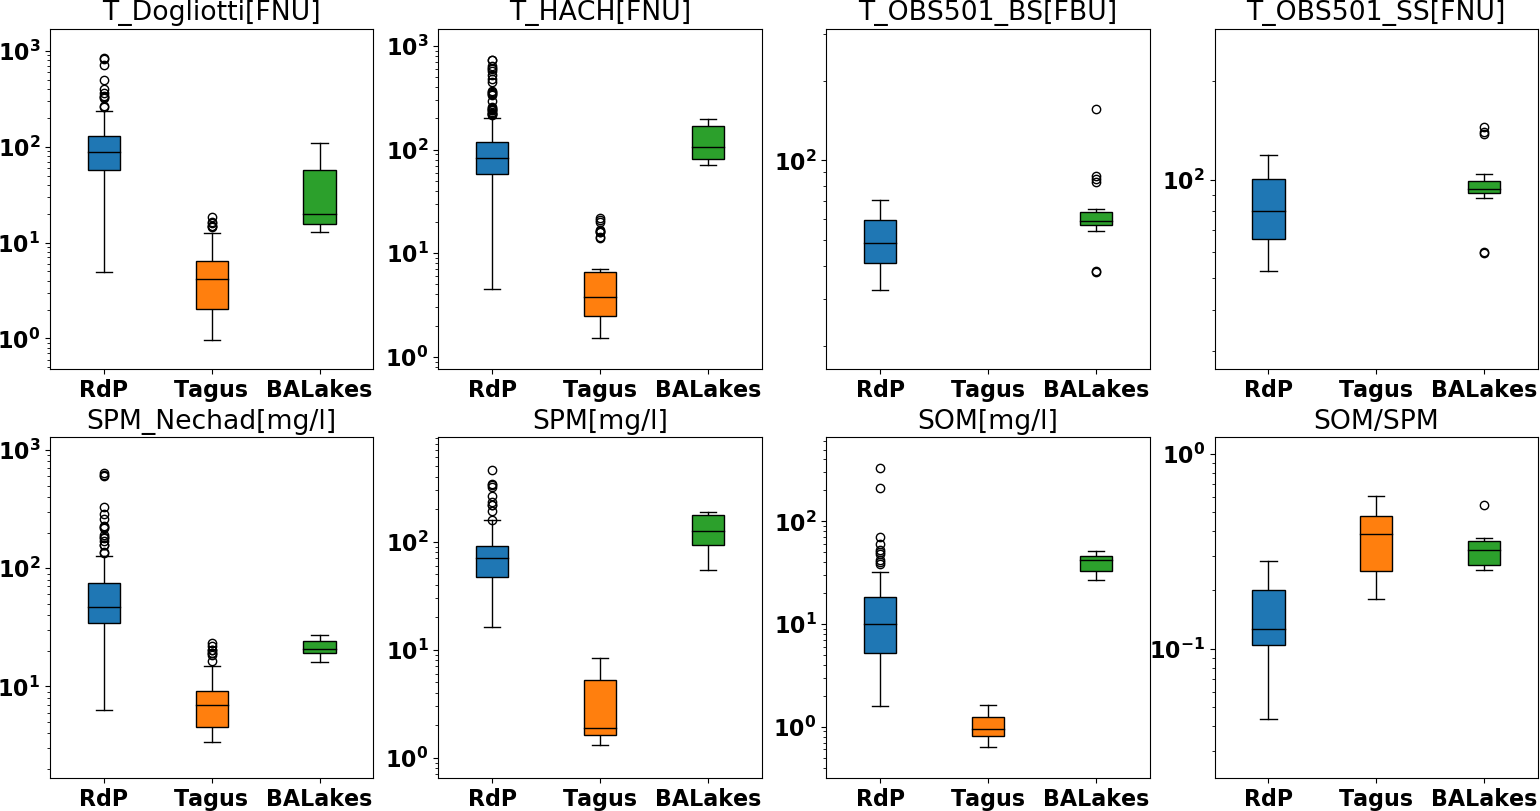
\includegraphics[width=\textwidth]{dat/figures/boxplot.png}
        \caption[Diagramas de cajas de las variables de campo no espectrales según región: Río de la Plata, Laguna de Chascomús y Río Tajo.]{Diagramas de cajas de las variables de campo no espectrales analizadas en este capítulo, divididas según región: Río de la Plata (RdP), Río Tajo (Tagus) y Laguna de Chascomús (BALakes).}
        \label{dat:boxplot}
        \end{figure}

        Prosiguiendo con el análisis, se eligieron algunas combinaciones de a pares de las variables no espectrales mencionadas cuya relación resulta de interés. Para estudiar dicha relación, se evaluó la linealidad entre las variables de dichos pares mediante el regresor lineal no paramétrico de Theil-Sen (Sen 1968, \cite{sen1968}, Theil et al. 1992, \cite{theil1992}). Dicho regresor difiere del convencional de cuadrados mínimos dado que está construido utilizando medianas, es decir, que será menos sensible a la presencia de anomalías. El Cuadro \ref{dat:tab:noespectrales} resume los resultados obtenidos para todos los pares de magnitudes considerados.

        La Figura \ref{dat:T_DogliottivsT_HACH} muestra la relación entre la turbidez estimada por el algoritmo de Dogliotti et al. 2015 (Ec. \ref{dat:eq:dogliotti2015}) y la medida \textit{in situ} por el HACH. Se observa una muy buena correspondencia entre sendas variables tanto para el RdP como para el Estuario del Tajo con pendientes y coeficientes de correlación cercanos a 1 y sesgos bajos. Teniendo en cuenta estas dos regiones, el algoritmo estima valores de turbidez con buena precisión en un rango dinámico de tres órdenes de magnitud [1 - 1000] FNU. En cuanto a la Laguna de Chascomús, si bien la correlación es alta, la estimación no resulta tan adecuada en términos globales (pendiente de $0.69$, sesgo de $-36.82$ FNU), resultando en una subestimación general de la turbidez. Interpretamos que esto ocurre para estas aguas debido a la fuerte presencia de pigmentos absorbentes en la banda roja de 645 nm (una de las utilizadas por el algoritmo de Dogliotti et al. 2015, Ec. \ref{dat:eq:dogliotti2015}). Dicho algoritmo fue calibrado con datos de campo de aguas moderada a altamente turbias; pero los sitios altamente turbios utilizados (RdP, Girondo y Guyana Francesa) no poseen tanto fitoplancton como la Laguna de Chascomús; por lo que sería necesario pensar una recalibración del algoritmo para contemplar estos escenarios, o bien redeterminar el régimen de transición lineal entre las bandas del rojo y la del NIR (llamado $\omega$ en Ec. \ref{dat:eq:dogliotti2015}).

        \begin{figure}
        \centering
        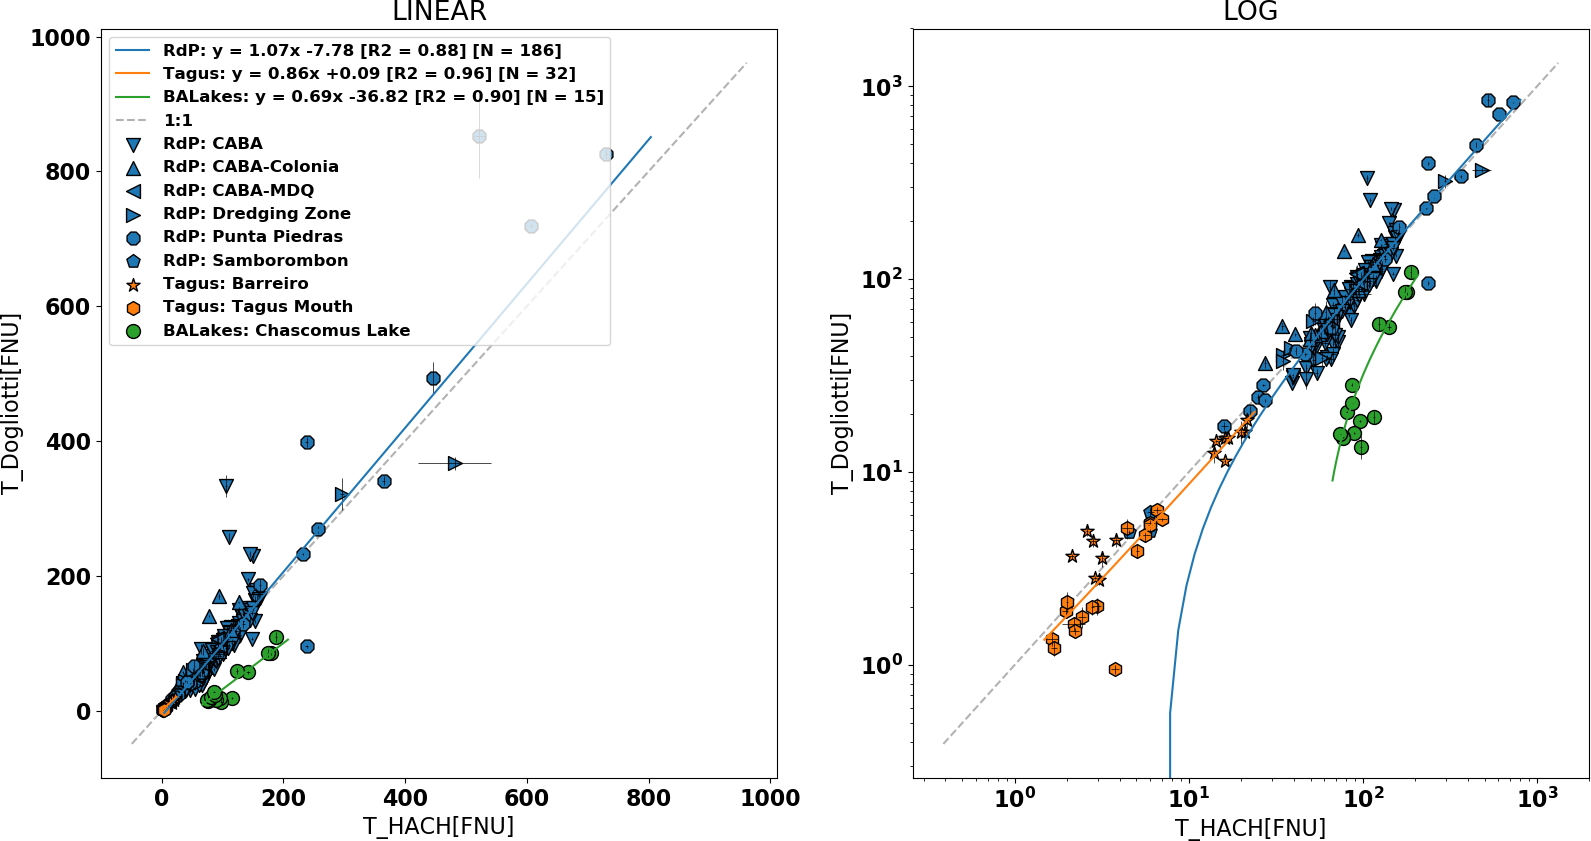
\includegraphics[width=\textwidth]{dat/figures/ScatterT_DogliottivsT_HACH.png}
        \caption[Relación entre la turbidez estimada a partir de reflectancias de agua de campo (T\_Dogliotti) vs. turbidez medida con el turbidímetro HACH.]{Relación entre la turbidez estimada a partir de reflectancias de campo (T\_Dogliotti) vs. turbidez medida con el turbidímetro HACH para las regiones consideradas. Escalas lineal (a) y logarítmica (b). El ajuste lineal fue hecho mediante el regresor no paramétrico de Theil-Sen (insensible a anomalías).}
        \label{dat:T_DogliottivsT_HACH}
        \end{figure}

        El resultado de la validación del algoritmo de una banda de Nechad et al. 2010 utilizado para determinar SPM es muy diferente al anterior (Figura \ref{dat:SPM}), dado que en este caso la correlación entre los valores observados (SPM) y estimados (SPM\_Nechad) resulta muy baja para valores altos de SPM. El coeficiente de correlación para el caso del RdP resultó de $R^{2}=0.02$, y si bien el mismo da razonablemente alto para la Laguna de Chascomús ($R^{2}=0.89$), la pendiente y el sesgo obtenidos están muy alejados del par ideal $(1;\,0\,mg/l)$ - resultó $(0.07;\,13.78\,mg/l)$. El único sitio considerado donde el estimador de Nechad et al. 2010 da buenos resultados es el Estuario del Tajo (pendiente de $0.93$, sesgo de $2.40$ $mg/l$ y correlación de $R^{2}=0.94$). Dicho comportamiento general era esperable, dado que el algoritmo fue diseñado con la banda del rojo en aguas dominadas por partículas minerales. En las aguas del RdP, dicha banda \textit{satura}, es decir que alcanza un comportamiento asintótico que se traduce en una baja sensibilibilidad del algoritmo para detectar diferencias de SPM. Por otro lado, al igual que lo ocurrido con el algoritmo de turbidez, en las aguas de la Laguna de Chascomús dicha banda se halla dominada por el efecto de la absorción del fitoplancton, lo que se traduce en una subestimación de la dispersión de partículas, implicando una subestimación sistemática en los valores de SPM.

        \begin{figure}
        \centering
        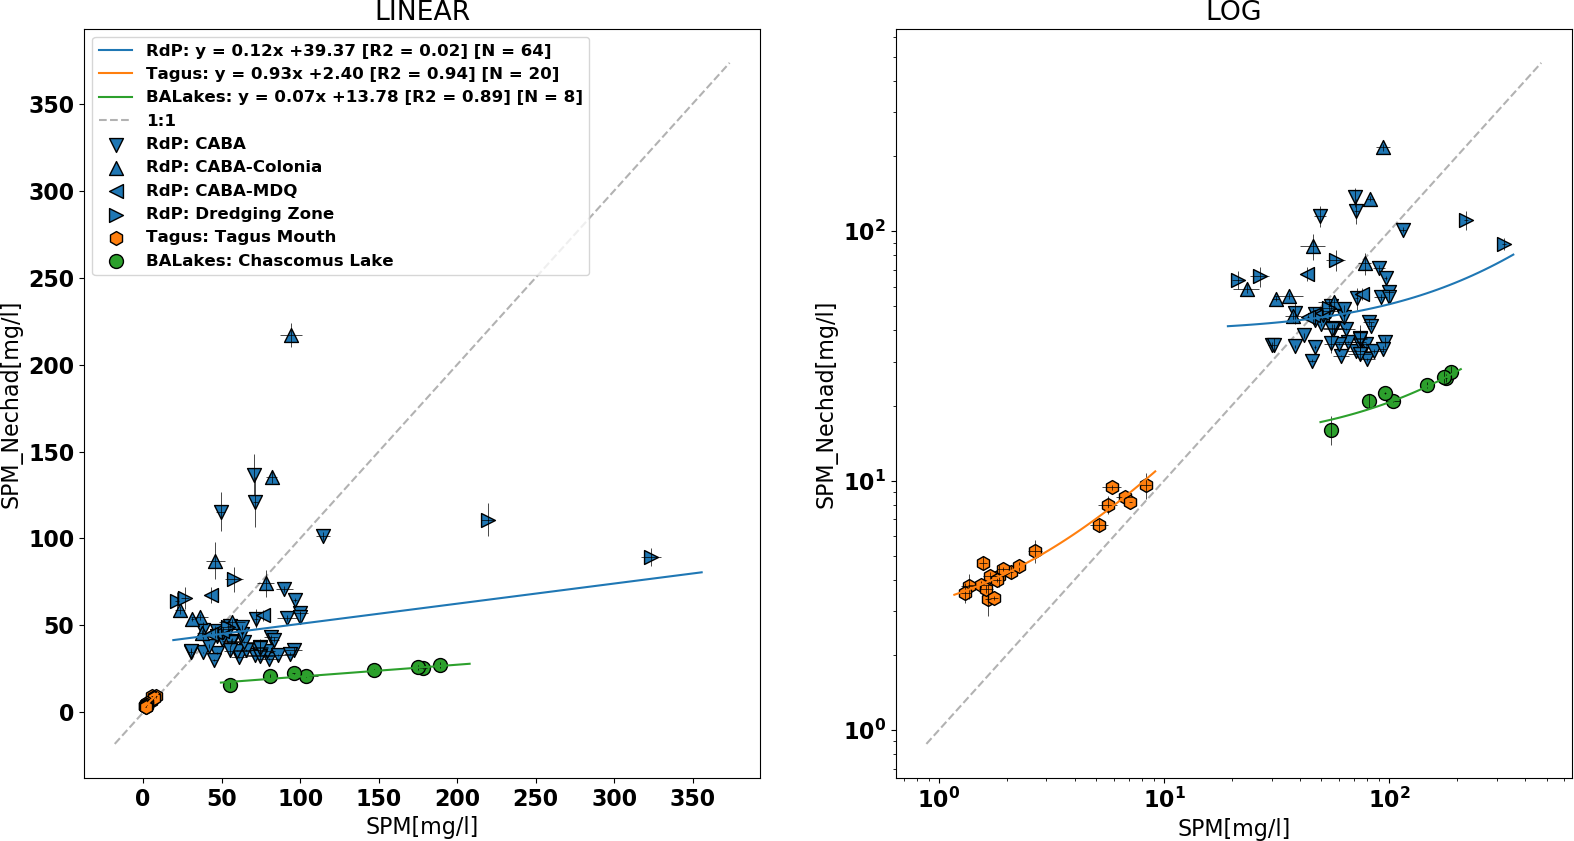
\includegraphics[width=\textwidth]{dat/figures/ScatterSPM_NechadvsSPM.png}
        \caption[Relación entre la concentración de material particulado en suspensión a partir de reflectancias de campo (SPM\_Nechad) y medido \textit{in situ}.]{Ídem Figura \ref{dat:T_DogliottivsT_HACH} pero para la relación entre la concentración de material particulado en suspensión a partir de reflectancias de campo (SPM\_Nechad) y medido \textit{in situ}.}
        \label{dat:SPM_NechadvsSPM}
        \end{figure}
        
        Por otro lado, aparte de considerar el cociente de material orgánico y total ($SOM/SPM$) individual por estación y evaluar su rango de variabilidad (Figura \ref{dat:boxplot}), se obtuvieron valores representativos de dicha fracción mediante una regresión lineal con ordenada nula para cada región (Figura \ref{dat:SOMvsSPM}). Dichas regresiones muestran una fracción de materia orgánica elevada en los casos de Chascomús y Tajo ($32\%$ y $39\%$) y baja en el caso del RdP ($13\%$). Es importante destacar que \textit{a priori} era esperable hallar un comportamiento variable para dicha fracción dentro del RdP, pero de la Figura \ref{dat:SOMvsSPM} no se evidencian diferentes regímenes al considerar las diferentes subregiones (\textit{CABA}, \textit{CABA-Colonia}, etc.).

        \begin{figure}
        \centering
        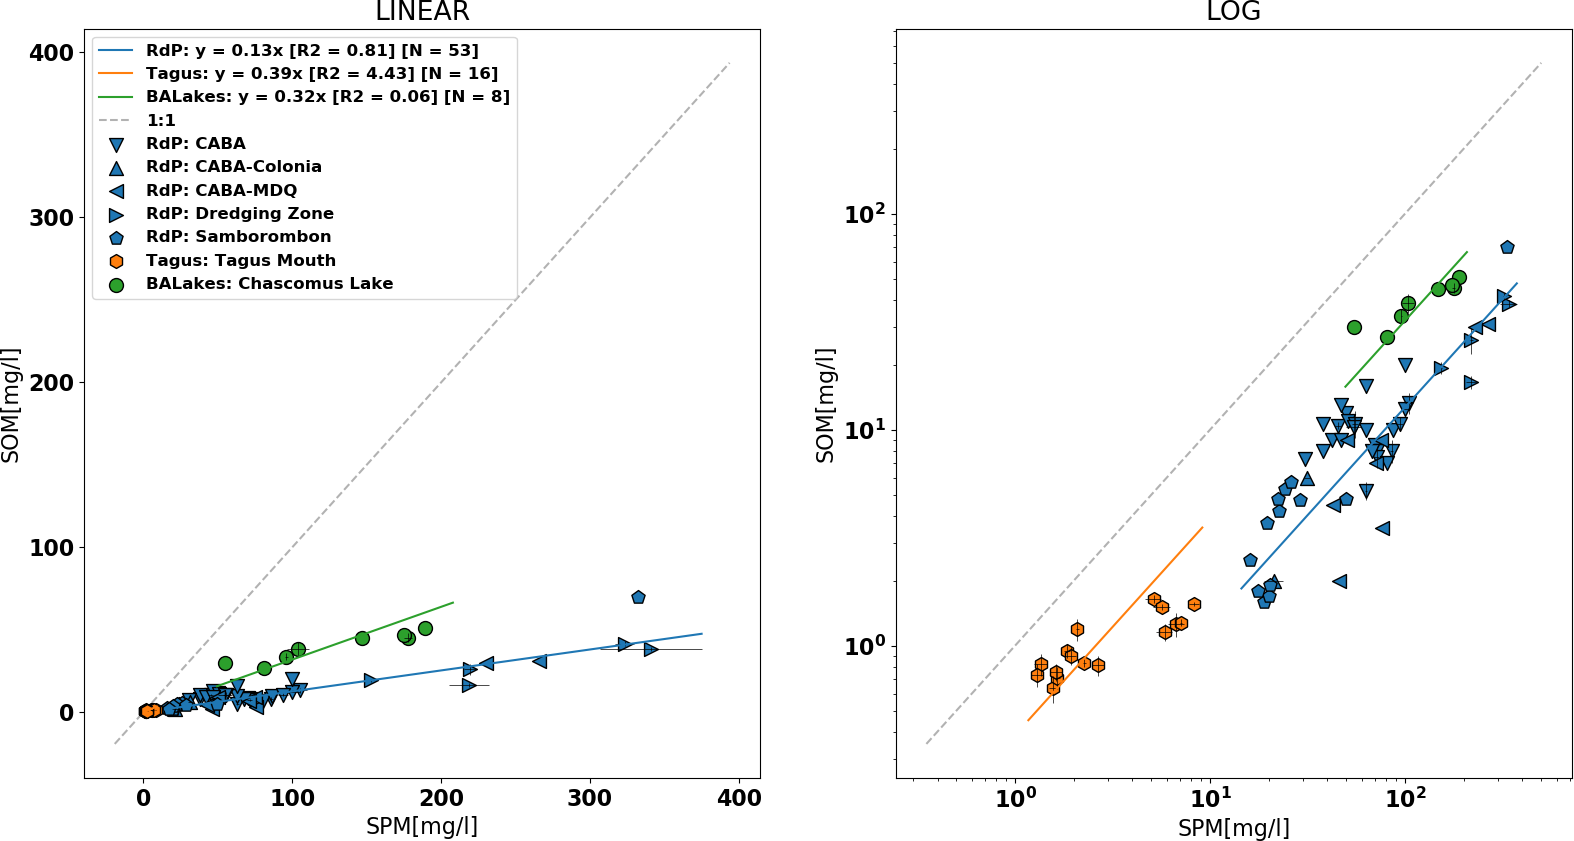
\includegraphics[width=\textwidth]{dat/figures/ScatterSOMvsSPM.png}
        \caption[Relación entre las concentraciones de material particulado en suspensión orgánico (SOM) vs. total (SPM).]{Ídem Figura \ref{dat:T_DogliottivsT_HACH} pero para la relación entre las concentraciones de material particulado en suspensión orgánico (SOM) vs. total (SPM).}
        \label{dat:SOMvsSPM}
        \end{figure}
        
        Como bien es descrito en Dogliotti et al. 2015, \cite{dogliotti2015} (véanse también Moreira et al. 2013, \cite{moreira2013}, Novoa et al. 2017, \cite{novoa2017}, entre otros), la relación entre la turbidez y el SPM muestra una gran variabilidad de un lugar a otro dependiendo de la naturaleza, la forma y el tamaño de las partículas. Por ejemplo, Gohin 2011, \cite{gohin2011}, encuentra una pendiente de $1.85$ FNU.l/mg para las áreas de Dunkerque y Boulogne (sur del Mar del Norte y al este del Canal de la Mancha); Snedden et al. 2007, \cite{snedden2007}, reportan una pendiente de $0.89$ FNU.l/mg para el estuario de Breton (río Mississippi), y Petus et al. 2010, \cite{petus2010}, estiman un valor de $0.74$ FNU.l/mg en las aguas de la costa vasca (Río Adour). Este valor coincide con el hallado por nosotros para el RdP de $0.74$ FNU.l/mg, que a su vez es muy similar al hallado previamente por Moreira et al. 2013 para esta región, de $0.73$ FNU.l/mg. Tanto para el Tajo como para Chascomús, dicho coeficiente es mayor ($0.89$ FNU.l/mg y $1.00$ FNU.l/mg, resp.). Si bien dicha relación es un parámetro distintivo del tipo (tamaño y composición) de partículas presentes en cada uno de los cuerpos de agua considerados, un análisis exhaustivo que pretenda explicar dichas diferencias excede los propósitos de esta tesis.

        \begin{figure}
        \centering
        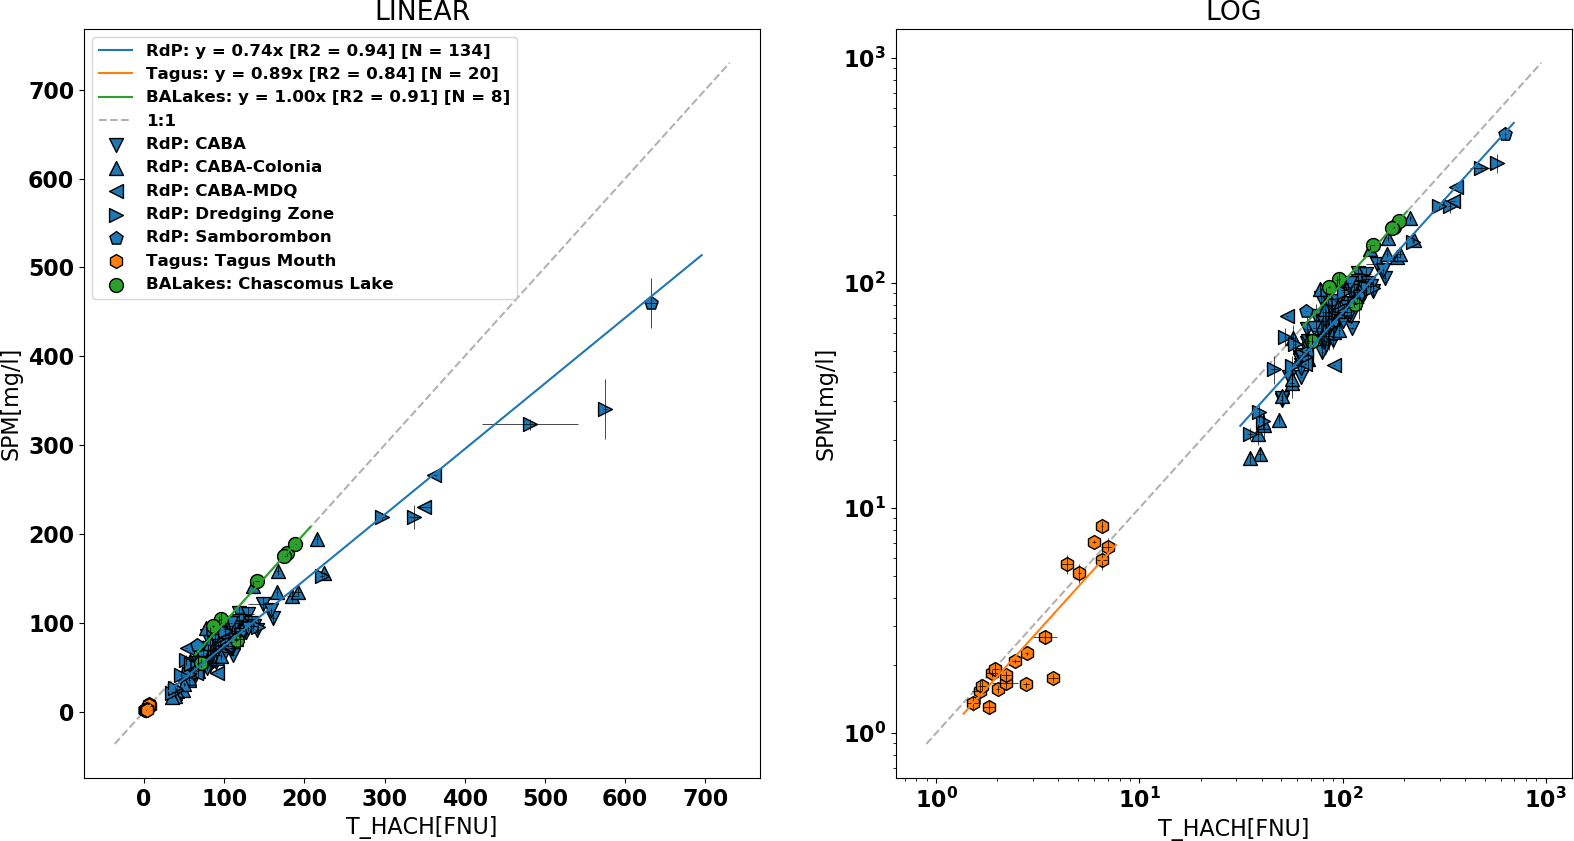
\includegraphics[width=\textwidth]{dat/figures/ScatterSPMvsT_HACH.png}
        \caption[Relación entre SPM y turbidez medida por el turbidímetro HACH.]{Ídem Figura \ref{dat:T_DogliottivsT_HACH} pero para la relación entre SPM y turbidez medida por el turbidímetro HACH.}
        \label{dat:SPMvsT_HACH}
        \end{figure}
        
        Por último, se comparan, a modo de caracterización, las relaciones entre los valores de turbidez obtenidos para cada uno de los medidores de turbidez utilizados (Figuras \ref{dat:T_OBS501_SSvsT_OBS501_BS} y \ref{dat:T_OBS501_SSvsT_HACH}). Se observa una relación lineal entre T\_OBS501\_BS y T\_OBS501\_SS (retrodispersómetro y nefelómetro del OBS501), aunque no se observan diferencias significativas en dicha relación al comparar el RdP con la Laguna de Chascomús (no hay datos de OBS501 disponibles para el Estuario del Tajo), con pendientes de $1.84$ FBU/FNU y $1.71$ FBU/FNU y sesgos de $1.84$ FBU y $1.71$ FBU. Por otro lado, los valores de $T\_OBS501\_SS$ y $T\_HACH$ se asemejan fuertemente para la región del RdP (pendiente $0.91$ FNU/FNU, sesgo $8.56$ FNU y correlación $0.92$), sin embargo presentan fuertes diferencias para la Laguna de Chascomús (pendiente $0.46$ FNU/FNU, sesgo $57.42$ FNU y correlación $0.81$). Si bien el número de puntos que se dispone para Chascomús no es suficiente [$N = 17$] para brindar un resultado conclusivo, también es cierto que \textit{a priori} dichos valores no tienen que coincidir, dado que son medidos mediante métodos diferentes a pesar de tener las mismas unidades: las fuentes son levemente diferentes y aparte el OBS501\_SS es un nefelómetro mientras que el HACH 2100Q \textit{is} es un turbidímetro.
        
        \begin{figure}
        \centering
        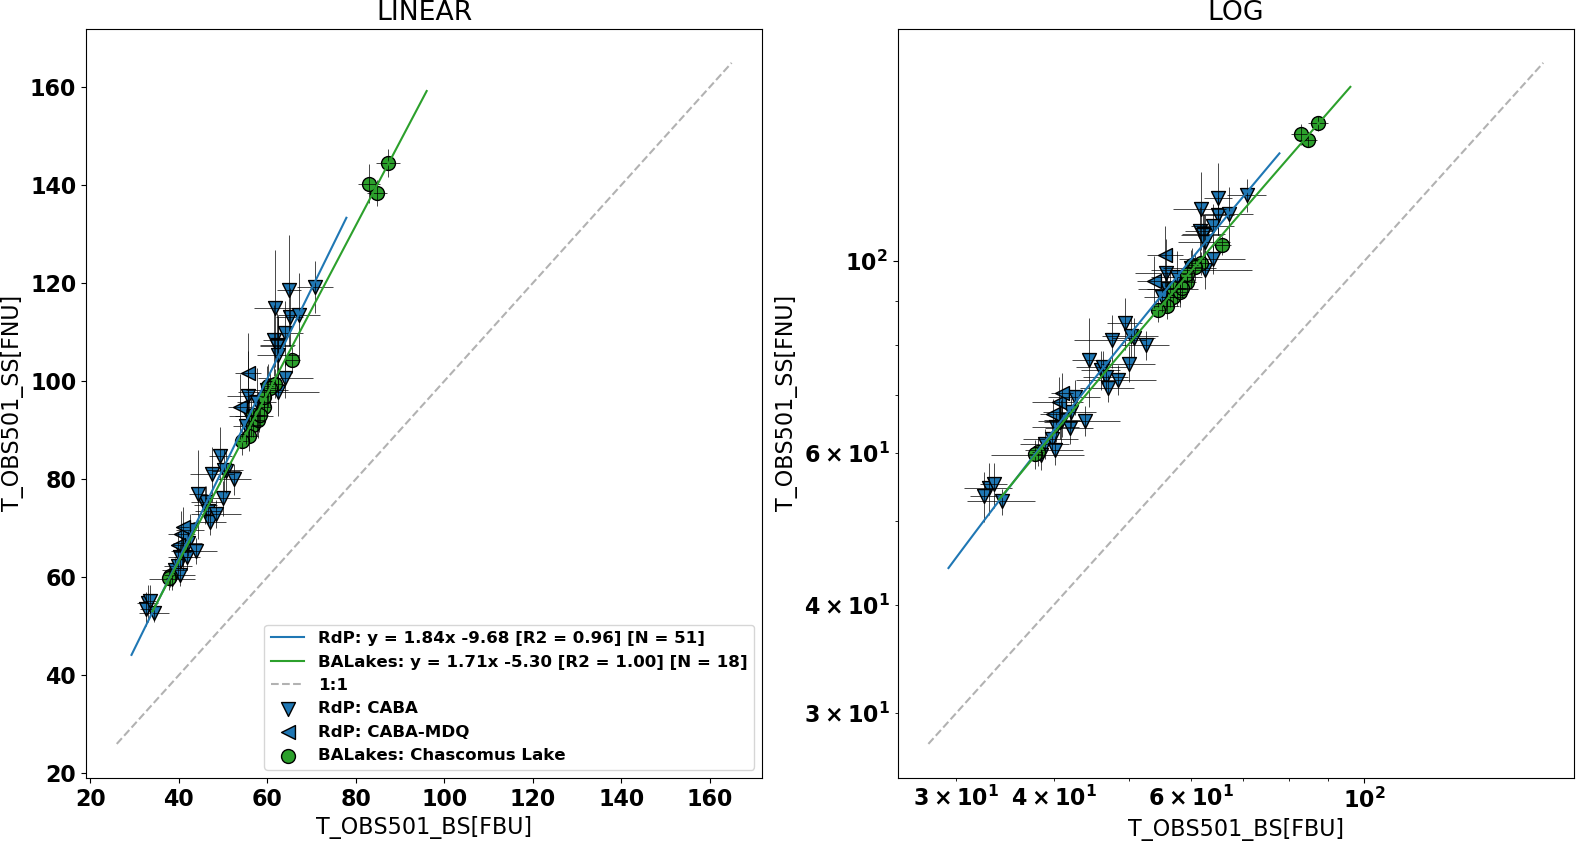
\includegraphics[width=\textwidth]{dat/figures/ScatterT_OBS501_SSvsT_OBS501_BS.png}
        \caption{Ídem Figura \ref{dat:T_DogliottivsT_HACH} pero para la relación entre la turbidez medida por el nefelómetro (T\_OBS501\_SS) vs. el retrodispersómetro (T\_OBS501\_BS) del OBS501.}
        \label{dat:T_OBS501_SSvsT_OBS501_BS}
        \end{figure}
        
        \begin{figure}
        \centering
        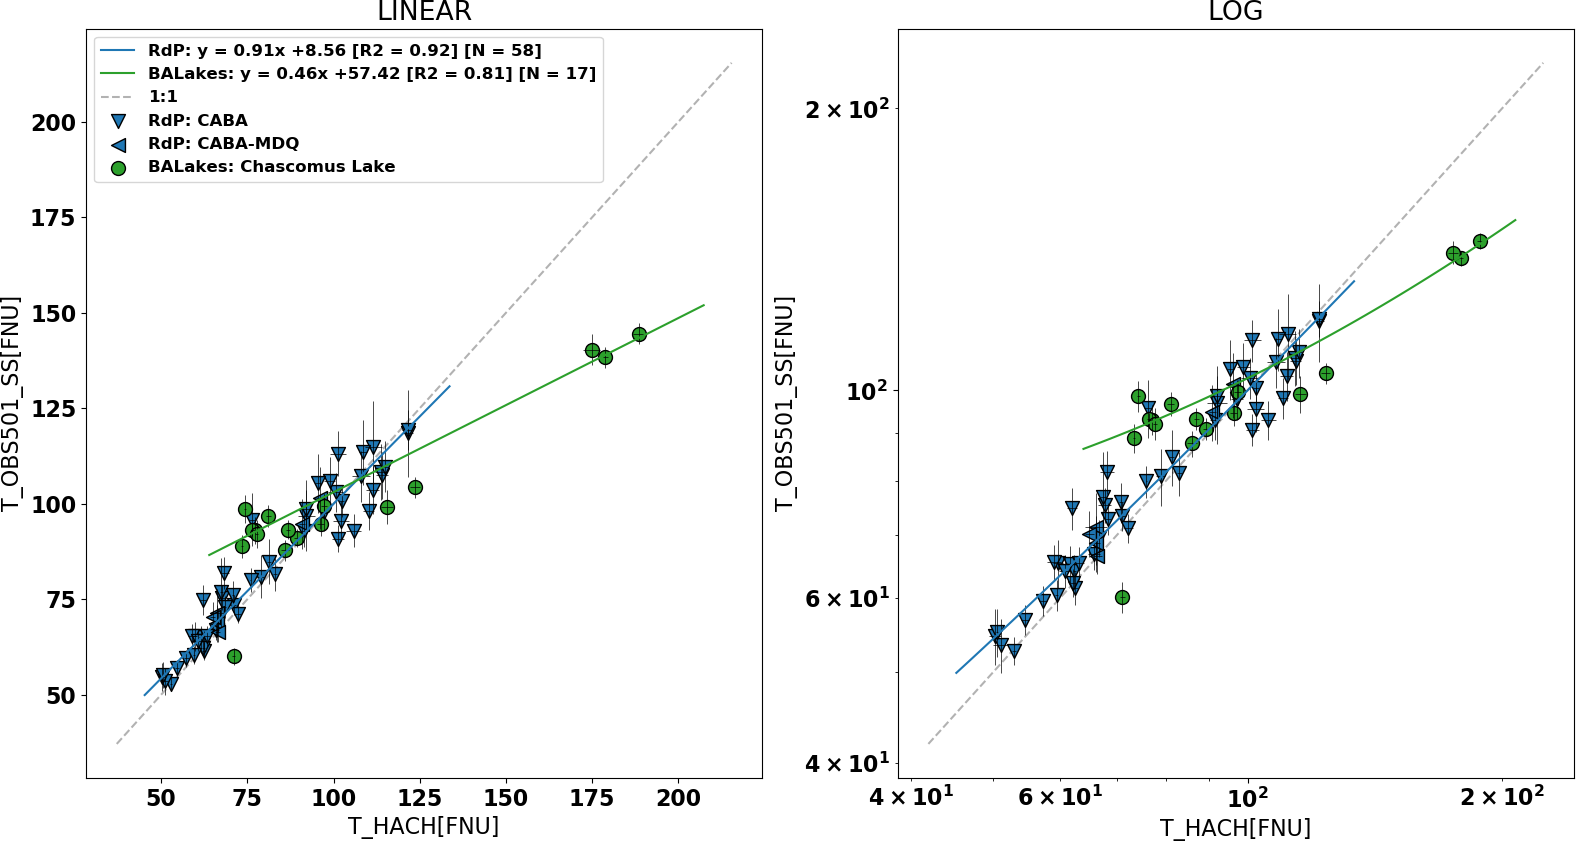
\includegraphics[width=\textwidth]{dat/figures/ScatterT_OBS501_SSvsT_HACH.png}
        \caption[Relación entre valores de turbidez medidos con el nefelómetro sumergible (T\_OBS501\_SS) y el turbidímetro portátil (T\_HACH).]{Ídem Figura \ref{dat:T_DogliottivsT_HACH} pero para la relación entre valores de turbidez medidos por el nefelómetro sumergible (T\_OBS501\_SS) y el turbidímetro portátil (T\_HACH).}
        \label{dat:T_OBS501_SSvsT_HACH}
        \end{figure}

        \begin{table}
        \caption[Resultados obtenidos para las regresiones lineales para cada uno de los pares de variables de campo medidas y regiones de estudio.]{Resultados - pendiente, sesgo, coeficiente de correlación, desviación absoluta mediana (MAD, Ec. \ref{ppe:eq:mad}) - obtenidos para las regresiones lineales no paramétricas (Regresor de Theil-Sen) para cada uno de los pares de variables y regiones de estudio.}
        \small
        \begin{tabular}{|c|l|l|l|l|l|l|}
        \hline
        \multicolumn{1}{|l|}{\textbf{Variables}}                                                                                 & \textbf{Región}                         & \textbf{Pendiente}          & \textbf{Sesgo}                & \textbf{R2}                  & \textbf{MAD} & \textbf{N} \\ \hline
                                                                                                                                 & {\color[HTML]{3531FF} \textbf{RdP}}     & 1.07                        & -7.78                         & 0.877                        & 45.30        & 186        \\ \cline{2-7} 
                                                                                                                                 & {\color[HTML]{F56B00} \textbf{Tagus}}   & 0.86                        & 0.09                          & 0.956                        & 3.05         & 32         \\ \cline{2-7} 
        \multirow{-3}{*}{\textbf{\begin{tabular}[c]{@{}c@{}}T\_Dogliotti{[}FNU{]}\\ vs.\\ T\_HACH{[}FNU{]}\end{tabular}}}        & {\color[HTML]{009901} \textbf{BALakes}} & {\color[HTML]{FE0000} 0.69} & {\color[HTML]{FE0000} -36.82} & 0.899                        & 23.51        & 15         \\ \hline
                                                                                                                                 & {\color[HTML]{3531FF} \textbf{RdP}}     & {\color[HTML]{FE0000} 0.12} & {\color[HTML]{FE0000} 39.37}  & {\color[HTML]{FE0000} 0.020} & 10.48        & 64         \\ \cline{2-7} 
                                                                                                                                 & {\color[HTML]{F56B00} \textbf{Tagus}}   & 0.93                        & 2.40                          & 0.939                        & 1.06         & 20         \\ \cline{2-7} 
        \multirow{-3}{*}{\textbf{\begin{tabular}[c]{@{}c@{}}SPM\_Nechad{[}mg/l{]}\\ vs.\\ SPM{[}mg/l{]}\end{tabular}}}           & {\color[HTML]{009901} \textbf{BALakes}} & {\color[HTML]{FE0000} 0.07} & {\color[HTML]{FE0000} 13.78}  & 0.893                        & 3.45         & 8          \\ \hline
                                                                                                                                 & {\color[HTML]{3531FF} \textbf{RdP}}     & 0.74                        & 0 (fijo)                      & 0.941                        & 28.53        & 134        \\ \cline{2-7} 
                                                                                                                                 & {\color[HTML]{F56B00} \textbf{Tagus}}   & 0.89                        & 0 (fijo)                      & 0.836                        & 1.33         & 20         \\ \cline{2-7} 
        \multirow{-3}{*}{\textbf{\begin{tabular}[c]{@{}c@{}}SPM{[}mg/l{]}\\ vs.\\ T\_HACH{[}FNU{]}\end{tabular}}}                & {\color[HTML]{009901} \textbf{BALakes}} & 1.00                        & 0 (fijo)                      & 0.908                        & 42.95        & 8          \\ \hline
                                                                                                                                 & {\color[HTML]{3531FF} \textbf{RdP}}     & 0.91                        & 8.56                          & 0.923                        & 19.14        & 58         \\ \cline{2-7} 
                                                                                                                                 & {\color[HTML]{F56B00} \textbf{Tagus}}   &                             &                               &                              &              &            \\ \cline{2-7} 
        \multirow{-3}{*}{\textbf{\begin{tabular}[c]{@{}c@{}}T\_OBS501\_SS{[}FNU{]}\\ vs.\\ T\_HACH{[}FNU{]}\end{tabular}}}       & {\color[HTML]{009901} \textbf{BALakes}} & {\color[HTML]{FE0000} 0.46} & {\color[HTML]{FE0000} 57.42}  & 0.812                        & 8.99         & 17         \\ \hline
                                                                                                                                 & {\color[HTML]{3531FF} \textbf{RdP}}     & 1.84                        & -9.68                         & 0.955                        & 18.64        & 51         \\ \cline{2-7} 
                                                                                                                                 & {\color[HTML]{F56B00} \textbf{Tagus}}   &                             &                               &                              &              &            \\ \cline{2-7} 
        \multirow{-3}{*}{\textbf{\begin{tabular}[c]{@{}c@{}}T\_OBS501\_SS{[}FNU{]}\\ vs.\\ T\_OBS501\_BS{[}FBU{]}\end{tabular}}} & {\color[HTML]{009901} \textbf{BALakes}} & 1.71                        & -5.30                         & 0.995                        & 10.13        & 18         \\ \hline
                                                                                                                                 & {\color[HTML]{3531FF} \textbf{RdP}}     & 0.13                        & 0 (fijo)                      & 0.812                        & 5.16         & 53         \\ \cline{2-7} 
                                                                                                                                 & {\color[HTML]{F56B00} \textbf{Tagus}}   & 0.39                        & 0 (fijo)                      & 4.430                        & 0.62         & 16         \\ \cline{2-7} 
        \multirow{-3}{*}{\textbf{\begin{tabular}[c]{@{}c@{}}SOM{[}mg/l{]}\\ vs.\\ SPM{[}mg/l{]}\end{tabular}}}                   & {\color[HTML]{009901} \textbf{BALakes}} & 0.32                        & 0 (fijo)                      & 0.062                        & 14.08        & 8          \\ \hline
        \end{tabular}
        \label{dat:tab:noespectrales}
        \end{table}

\section{Conclusiones}
\label{dat:s:conclusiones}
    
    En este capítulo se presentaron los datos de campo disponibles para el área de estudio de la presente tesis - el RdP - y se los comparó con datos bioópticos obtenidos en otras áreas de estudio exploradas por nuestro grupo de investigación - el estuario del Tajo en Portugal y la Laguna de Chascomús en la Provincia de Buenos Aires - con el fin de extraer similitudes y rasgos distintivos de las mediciones del RdP. Dichas regiones de estudio difieren ópticamente del RdP esencialmente en concentración (Tajo) y en contenido de material orgánico (Tajo y Chascomús). Se exhibió la distribución geográfica de las estaciones realizadas en en RdP y en dichas regiones y se hizo una descripción de cada una de las magnitudes medidas: reflectancias del agua mediante mediciones radiométricas (ASD y TriOS), turbidez mediante diferentes turbidímetros (HACH y OBS501) y determinación de la concentración de masa en volumen de material particulado en suspensión (SPM) mediante el método gravimétrico aplicado sobre muestras filtradas de agua. A su vez, se describieron los instrumentos utilizados, sus protocolos de medición y procesamiento. También, a partir de las reflectancias del agua, se computaron los algoritmos de turbidez de Dogliotti et al. 2015, \cite{dogliotti2015}, y de SPM de Nechad et al. 2010, \cite{nechad2010} para poder validar dichos algoritmos en nuestra región de estudio.
    
    Por otro lado, se describió el método que fue utilizado para sistematizar los datos de campo en una base de datos relacional, para lo cual fue necesario organizar los datos en forma de campos y entradas con una llave identificatoria única (estaciones). La sistematización de la base de datos - incluyendo la realización de los códigos para procesar los datos adquiridos durante las campañas - y el análisis de los mismos se realizó mediante el módulo \textit{pandas} del lenguaje \textit{Python}, cuyo desempeño resultó óptimo en nuestro caso, dado que es un lenguaje de alto nivel - es decir, intuitivo pero no necesariamente el más veloz - y a su vez el volumen de datos no excede los tamaños recomendables para \textit{pandas} ($\approx 50 GB$). En caso de que la base de datos continúe expandiéndose (por ej. aumentar en un factor 10 ó más su tamaño) será necesario abordar los datos con lenguajes específicos de bases de datos, como \textit{SQL} (\textit{Structured Query Language}). Los principales códigos generados para procesar, sistematizar y analizar los datos de campo se hallan en \href{https://github.com/juanchossn/scripts_tesis_doctoral}{\textbf{\underline{este repositorio}}}\cite{repo}.
    
    Los resultados obtenidos para el conjunto total de las mediciones son compatibles con lo esperado. Se observan rasgos espectrales distintivos del RdP con respecto al Tajo y a Chascomús: valores de reflectancias en el rojo/NIR/SWIR más elevados que en Tajo y Chascomús; un impacto marcadamente menor debido a la absorción de pigmentos fotosintéticos, y al igual que en Tajo y Chascomús, una elevada correlación negativa entre la forma espectral de las reflectancias y la absorción del agua en el rojo/NIR/SWIR.
    Por otro lado, se observan valores típicos de turbidez y SPM similares entre el RdP y la Laguna de Chascomús ($\approx 80$ FNU y $\approx 80$ mg/l), a su vez marcadamente mayores a los observados en el Estuario del Tajo ($\approx 5$ FNU y $\approx 2$ mg/l). Asimismo, se observan fracciones de material orgánico a total (SOM/SPM) menores en el RdP ($13\%$) en comparación con Chascomús y Tajo ($32\%$ y $39\%$, respectivamente), situación ya discernible del análisis de las diferencias entre las firmas espectrales ya descritas. A su vez, se observa una relación entre la turbidez (FNU, HACH) y SPM en el RdP de $0.74$ FNU.l/mg, muy similar a la ya encontrada por Moreira et al. 2013 de $0.73$ FNU.l/mg para nuestra región de estudio.
    
    Los valores de turbidez estimados por el algoritmo de Dogliotti et al. 2015 son plausibles tanto para el RdP como para el Tajo, abarcando un rango dinámico de 1-1000 FNU; mientras que subestiman los observados en Chascomús. Dicha discrepancia está asociada a un marcado impacto de la absorción de fotopigmentos en la banda del rojo (utilizada por el algoritmo en regímenes de turbidez baja a moderada). El mismo efecto de subestimación se observa al evaluar la estimación de SPM por el algoritmo de Nechad et al. 2010 para la región de Chascomús; aunque este algoritmo tampoco estima bien los valores de SPM en regímenes de altas concentraciones del RdP ($R^{2}=0.02$), resultado esperable dado que no incorpora la transición al NIR para evadir la saturación que sí incorpora el de Dogliotti et al. 2015 para regímenes de turbidez/SPM altos.
    
    Finalmente, se estudiaron las relaciones entre los valores de turbidez estimados por los diferentes medidores de turbidez descritos (turbidímetro HACH y retrodispersómetro y nefelómetro OBS501). Se observan comportamientos lineales con baja ordenada al origen para la relación entre el nefelómetro y el retrodispersómetro del OBS501, sin observarse diferencias significativas entre regiones. Si bien las mediciones de turbidez por dispersión a $90\degree$ del OBS501 y del HACH (ambas en unidades nefelométricas de formazina, FNU, y dentro de los requerimientos de la ISO 7027) son consistentes para el RdP (pendiente de 0.91 FNU/FNU, sesgo de 8.56 FNU y correlación de $R^{2}=0.92$), presentan diferencias significativas en las aguas de la Laguna de Chascomús (pendiente de 0.46 FNU/FNU, sesgo de 57.42 FNU y correlación de $R^{2}=0.81$). Si bien es cierto que se necesitarían más datos para evaluar mejor dicha correspondencia (actualmente, $N = 17$), también es cierto que, si bien ambas mediciones satisfacen los requerimientos de la ISO 7027 y están referidas a las mismas unidades, no son perfectamente comparables dados sus diferentes métodos de medición (turbidimétrico en caso del HACH y nefelométrico en caso del OBS501\_SS). Aún así, un análisis exhaustivo que pretenda explicar dicha discrepancia excede los objetivos de esta tesis.
    
    Las curvas de reflectancias presentadas y analizadas en este capítulo fueron utilizadas para calibrar y validar el algoritmo presentado en \S \ref{blr} y para validar el algoritmo presentado en \S \ref{pca}. El hecho de haber adquirido y sistematizado una base de datos de campo para las aguas ópticamente complejas del RdP es de un gran potencial para la calibración y validación de futuros algoritmos bioópticos desarrollados para nuestra región de interés.